\documentclass{my_memo}

\usepackage{booktabs}
\usepackage{tabularx}
\usepackage{siunitx}
\usepackage{microtype}
\usepackage{hyperref}
\sloppy

\title{Reproducing the Hensley \& Draine (2023) Astrodust SED}
\author{Kwang-il Seon}
\date{\docmoddate}

\newcommand{\Cabs}{\ensuremath{C_{\rm abs}}}
\newcommand{\Qabs}{\ensuremath{Q_{\rm abs}}}
\newcommand{\Qext}{\ensuremath{Q_{\rm ext}}}
\newcommand{\Qsca}{\ensuremath{Q_{\rm sca}}}
\newcommand{\Teq}{\ensuremath{T_{\rm eq}}}
\newcommand{\Nh}{\ensuremath{N_{\rm H}}}
\newcommand{\lamIlam}{\ensuremath{\lambda I_\lambda}}
\newcommand{\fc}{\ensuremath{f_{C}^{\text{vol}}}}
\newcommand{\umass}{\ensuremath{\,\mu{\rm m}}}
\newcommand{\HD}[1]{HD23~#1}

% The my_memo class (mathrsfs + amssymb + kotex + explicit
% \DeclareMathAlphabet for \mathbf/\mathit/\mathbit) sits at the 16
% math-family limit; using \mathbf here overflows it ("Too many math
% alphabets"). Route \mathbf through \boldsymbol, which reuses the bold
% math version instead of allocating a new family. Vectors and bold
% emphasis render the same to the eye (bold italic for letters).
\let\mathbf\boldsymbol

% Some upright multi-letter sub/superscripts containing a "v" are written
% \text{...} rather than {\rm ...}.  That was a workaround for the OLD
% kiseon_memo class, whose \DeclareMathSymbol{v}{\mathalpha}{ntxlettersA}{51}
% kept slot 51 while a math alphabet swapped the family, so inside \rm the
% slot was read from Times roman, where it is the digit 3 ($B_{\rm env}$ came
% out as "B_en3").  my_memo assembles the mathchar from the current family at
% run time and declares the glyph-to-Unicode mapping, so {\rm ...} is safe
% again and both spellings now typeset -- and extract from the PDF -- correctly.

\begin{document}
\maketitle

\section{Introduction}

This memo documents the construction of an astrodust thermal emission
pipeline that reproduces the Hensley \& Draine (2023, ApJ 948, 55;
hereafter HD23) ``astrodust'' model from first principles, working
from the published dielectric function (Draine \& Hensley
2021a, ApJ 909, 94, hereafter DH21a) and size distribution. The
deliverable is a Fortran library callable from a 3D radiative-transfer
driver per cell, with the per-H emission expressed in HD23 units
(\si{erg.s^{-1}.sr^{-1}} per H atom).

The pipeline consists of five phases:
\begin{itemize}
  \item[A.] Random-orientation T-matrix sweep on the DH21 native grid
        (169 sizes $\times$ 1762 wavelengths,
        \SIrange{1e-4}{3.981e4}{\micro\meter}) producing
        \Qabs($\lambda, a$), \Qsca($\lambda, a$), and the asymmetry
        parameter $g$. Longward of \SI{0.0912}{\micro\meter} the axis is
        DH21a's own 200-per-decade grid, 1129 points. Shortward of it
        the axis is the DH21 dielectric function's own energy nodes,
        632 points from \SIrange{14.0}{12398}{\electronvolt}, so the
        absorption edges tabulated there stay exact steps between
        adjacent grid points instead of being averaged into ramps. Each
        is a pair of nodes about $10^{-4}$ apart in relative energy,
        across which ${\rm Im}(n)$ jumps by $+211\%$ at Fe\,K
        (\SI{7124}{\electronvolt}), $+131\%$ at O\,K
        (\SI{538}{\electronvolt}), $+67\%$ at Fe\,L
        (\SI{724}{\electronvolt}) and $+30\%$ at C\,K
        (\SI{291}{\electronvolt}). One point is not a node: $0.0912\,(1-10^{-4})$, which is
        interpolated and is placed to resolve the Lyman-limit step of
        the \emph{radiation field} rather than anything in the grain
        (\S\ref{sec:euv}). The orientation-resolved (polarized) table
        is a separate product and stays on the 1129-wavelength axis.
  \item[B.] Optical-depth verification:
        $\tau_{\rm Ad}/N_H = \sum_a (dn_{\rm Ad}/N_H)\,\pi a^2\,\Qext$
        compared against HD23 \texttt{extinction.dat}.
  \item[C.] Two-stage enthalpy: silicate-only (Stage~1) and
        silicate~+~carbonaceous volume-weighted (Stage~2).
  \item[D.] Single-cell SED solver with dynamic $T$ grid per radius.
  \item[E.] SED verification against the HD23 release answer key.
\end{itemize}
Two refinements were implemented in addition: PAH emission via the
Draine \& Li (2007) DL07 cross sections, and polarization
via the dichroic-extinction formula of HD23 \S2.2. A
Python sidecar of the solver (Phase G) is provided for downstream
prototyping.

The optical-depth acceptance criterion is met to within 0.5\%; the
polarization check matches the HD23 release to within 0.07\% in every wavelength band
(both essentially perfect reproductions). The SED comparison
falls $7.6\%$ below the HD23 release in the
\SIrange[range-phrase=--,range-units=single]{30}{300}{\micro\meter}
FIR-peak band (median relative residual; $10.1\%$ at the
\SI{133}{\micro\meter} peak itself) after applying the corrected
Mathis 4000\,K dilution factor (1.65$\times 10^{-13}$ instead of the
literal Mathis~1983 $1\times 10^{-13}$; the original-Mathis variant
gives $14.3\%$). This residual is now \emph{resolved}
(\S\ref{sec:phaseE-resolution}): an energy-budget audit shows the HD23
\emph{release} is internally inconsistent --- its emitted
\texttt{irem} tables radiate 9.3\% (astrodust) and 3.2\% (PAH) more
than its own released \Cabs\ absorb from the same field --- whereas our
pipeline conserves energy to 0.15\%. The deficit equals HD23's own
emitted-vs-absorbed excess; its component-dependence rules out a
heating-field / $U$-convention offset and points to an
internal-vs-released cross-section vintage difference.


\section{Reference parameters}

Table~\ref{tab:ref} lists the HD23 best-fit parameters that we hold
fixed throughout this work. The first three lines define the
dielectric function file \texttt{index\_DH21Ad\_P0.20\_0.00\_1.400};
the rest determine size grids, dust mass, and the heating field.

\begin{table}[h]
\centering
\caption{Reference parameters (HD23 best fit).}
\label{tab:ref}
\begin{tabularx}{0.95\textwidth}{l c X}
\toprule
Quantity & Value & Source \\
\midrule
Porosity $\mathcal{P}$                    & 0.2                    & HD23 \S3.1 \\
Metallic Fe fraction $f_{\rm Fe}$         & 0                      & HD23 \S3.1 \\
Axial ratio $b/a$ (oblate)                 & 1.4                    & HD23 \S3.1 \\
Solid mass density $\rho_{\rm solid}$      & 3.42 g/cm$^3$          & DH21a Tab.~2 \\
Bulk mass density $\rho_{\rm Ad}$          & 2.74 g/cm$^3$          & $= \rho_{\rm solid}(1-\mathcal{P})$ \\
$M_{\rm Ad}/N_H$                           & 0.0092                 & DH21a Tab.~2 \\
Heating intensity $U$                      & $10^{0.2} \approx 1.585$ & HD23 \S2.3.1 \\
Radiation-field shape                      & Mathis 1983 ISRF, scaled by $U$ & HD23 \S2.3.1 \\
$a_{\rm eff}$ range                        & \SIrange{3.16e-4}{5.012}{\micro\meter} & DH21a, 169 points \\
$\lambda$ range                            & \SIrange{1e-4}{3.981e4}{\micro\meter} & $Q$-table grid, 1762 points; see \S\ref{sec:euv} \\
\quad above the Lyman limit                & \SIrange{0.0912}{3.981e4}{\micro\meter} & DH21a, 200 per decade, 1129 points \\
\quad below it                             & \SIrange{1e-4}{9.119e-2}{\micro\meter} & DH21a dielectric-function nodes, 633 points \\
$\lambda$ range, polarized table           & \SIrange{0.0912}{3.981e4}{\micro\meter} & orientation-resolved, 1129 points \\
\bottomrule
\end{tabularx}
\end{table}


\section{Optical cross sections}

\subsection{Two-track cross-section architecture}

HD23 treats the astrodust and PAH populations on \emph{separate} tracks
for their optical properties, and our pipeline mirrors that separation
verbatim:

\begin{itemize}
  \item \textbf{Astrodust}~(HD23 \S3.1) is a single composite oblate
        spheroid with the DH21a dielectric function. Its extinction,
        scattering, and polarization cross sections are computed via
        the modified-particle-form approximation (MPFA, three
        orientations of $C_E(0^\circ)$, $C_E(90^\circ)$, $C_H(90^\circ)$
        per HD23~\S2.2) of the random-orientation T-matrix code of
        Mishchenko et al.~(1996). The result is the
        \texttt{q\_DH21Ad\_*} table used throughout Phases A--E and
        F-2. Astrodust is the only population that contributes to
        polarized extinction or emission.
  \item \textbf{PAH}~(HD23 \S3.2) is treated as spherical and
        compositionally distinct ($\rho_{\rm PAH} = 2.0$~g/cm$^3$ vs
        $\rho_{\rm Ad} = 2.74$~g/cm$^3$). Its cross sections follow
        Draine \& Li~(2007) for the neutral and ionized branches,
        blended with the random-orientation graphite Mie cross section
        $C^{\rm gra}$ via the size-dependent weight $\xi_{\rm gra}(a)$
        of HD23~eq.~16. No T-matrix; spherical Mie throughout. HD23
        explicitly assumes PAH does not contribute to polarized
        extinction or emission.
\end{itemize}

The two-track structure is propagated through the rest of the
pipeline: astrodust uses the T-matrix Q tables and the full MPFA,
PAH uses the DL07 cross sections (Sect.~\ref{sec:pah}). The
present section is the astrodust track. The PAH track lives in
Sect.~\ref{sec:pah}.

\subsection{T-matrix engine and parallel sweep}

We use the Mishchenko et al.\ (1996) random-orientation T-matrix code. It
entered the tree as \texttt{tmd.lp.f} wrapped as a callable subroutine
\texttt{TMD\_ONE(AXI, LAM, MRR, MRI, EPS, NP, DDELT, NDGS,
QEXT, QSCA, WALB, ASYMM, IERR)}, a mechanical
conversion of the original main program: inline test-case inputs became
arguments, the size-distribution loop was removed (one $a$ per call),
file I/O was dropped, and \texttt{STOP} statements were replaced with
\texttt{IERR}~/~\texttt{RETURN}. A critical footgun: the original main
mutates the input \texttt{DDELT} (\texttt{DDELT~=~0.1*DDELT}); when
called from F90 with a \texttt{parameter} constant, the write traps as
SIGBUS on a read-only page. The wrapper copied to a local
\texttt{DDELT\_LOC} before mutating.

That f77 driver has since been rewritten as a modern-Fortran library under
\texttt{tmatrix/src/}, and the entry point is now
\texttt{tmatrix\_eval(work, a\_um, lambda\_um, nr, ki, options,
result)}. The only fixed-form file left is \texttt{lpd.f}, the linear-algebra
routines the solver calls. The library holds no \texttt{COMMON}, no
\texttt{EQUIVALENCE} and no mutable \texttt{SAVE}: every working array lives in
a caller-owned \texttt{tmatrix\_workspace\_t}, one active caller for each
workspace, and distinct workspaces may be evaluated concurrently. The
convergence tolerance is a component of an \texttt{intent(in)}
\texttt{tmatrix\_options\_t}, so the \texttt{DDELT} hazard above cannot recur.
Mishchenko's unmodified sources (\texttt{tmd.lp.f}, \texttt{tmd.par.f},
\texttt{ampld.lp.f}, \texttt{ampld.par.f}) are kept under
\texttt{tmatrix/reference/upstream/} so that each migrated routine stays
checkable line by line against its original; nothing there is compiled. The
transition is numerically inert: the $Q$ tables it produces are byte-identical
across it.

Convergence-failure fallbacks are implemented for $x = 2\pi a/\lambda
< 0.1$ (small-$x$ spheroidal Rayleigh polarizability ported from
Draine 1992 \texttt{sphero.f}) and $x > 50$ (geometric optics, $\Qext
\to 2$). The small-$x$ fallback uses the exact oblate-spheroid
depolarization factors $L_a$, $L_b = (1-L_a)/2$ averaged over random
orientation, and was found to remove a systematic 6\% under-prediction
that a naive Mie-sphere fallback produces in the dipole limit.

The timings that follow were taken on the 1129-wavelength axis, before
the grid was carried into the ionizing band; the sweep on the present
1762-wavelength axis has not been timed, and the 633 wavelengths it
adds all fall in the ultraviolet slice, which is the expensive one.
The full 169 by 1129 sweep takes 11 minutes single-threaded on
Apple Silicon. A bash work-queue driver
\texttt{run\_parallel.sh} dispatching $K = 32$ chunks across $N = 6$
workers reduces this to 2 minutes 18 seconds (4.8$\times$ speedup)
with bit-identical output (Tab.~\ref{tab:parallel}). Equal-jw-range
partitioning ($K = N$) gives almost no speedup because the UV slice
is T-matrix-bound and stalls the run; the work-queue pattern is the
essential ingredient.

\begin{table}[h]
\centering
\caption{Parallel-sweep walltime measurements, on the 1129-wavelength
axis.}
\label{tab:parallel}
\begin{tabular}{l c c c c}
\toprule
mode             & $N$ & $K$ & walltime & speedup \\
\midrule
serial           & 1   & 1   &       11~m~0~s &        1.0$\times$ \\
equal partition  & 6   & 6   &       9~m~59~s &        1.1$\times$ \\
work queue       & 6   & 32  & \bfseries 2~m~18~s & \bfseries 4.8$\times$ \\
\bottomrule
\end{tabular}
\end{table}

\subsection{Result}

\autoref{fig:q} shows \Qext\ and \Qabs\ at four representative grain
sizes spanning the full DH21 range. The classic transition from
Rayleigh-like dipole behavior at small $x$ (small grains or long
wavelengths) to the geometric-optics plateau at large $x$ is visible.
Verification of $\Qabs$ against the HD23 release table
\texttt{q\_DH21Ad\_P0.20\_Fe0.00\_1.400.dat.gz}, taken against the
mean of its jori = 1, 2, 3 columns, gives a median deviation of
$-0.04\%$ and a mean absolute deviation of $0.33\%$ across the
T-matrix-converged region ($x \in [0.01, 30]$). (That mean is not the
random-orientation average, which is
$\tfrac{1}{3}Q^{\rm jori=2} + \tfrac{2}{3}Q^{\rm jori=3}$; the two
coincide only in the Rayleigh limit, where jori~1 and jori~3 measure the
same $Q_\perp$.) The largest deviations, a few percent, sit at the top
of that $x$ range where the geometric-optics limit takes over, and carry
negligible weight in any SED integral.

\begin{figure}[h]
\centering
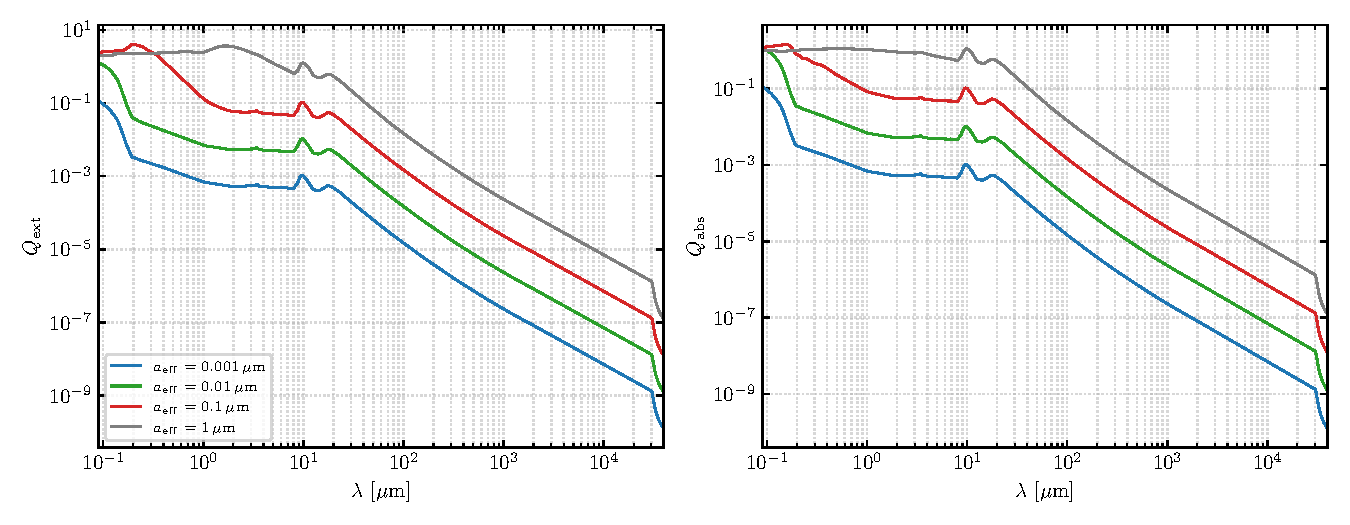
\includegraphics[width=0.95\textwidth]{figs/q_vs_lambda.pdf}
\caption{Extinction (left) and absorption (right) efficiency factors
as functions of wavelength for four representative grain sizes from
the DH21 grid. The transition from $Q \propto x^4$ scattering at long
wavelengths to $Q \to 1$ geometric optics at short wavelengths is
clearly resolved for each size.}
\label{fig:q}
\end{figure}


\section{Optical-depth verification}

The first end-to-end milestone is to verify that our cross
sections reproduce HD23's reported extinction per H atom:
\begin{equation}
\frac{\tau_{\rm Ad}}{N_H}\!\left(\lambda\right)
= \sum_a \frac{dn_{\rm Ad}}{N_H}\!\left(a\right) \,\pi a^2 \,\Qext(\lambda, a),
\label{eq:tau}
\end{equation}
where $(dn_{\rm Ad}/N_H)(a)$ is the HD23 size distribution
(\texttt{size\_distribution.dat} column~2), already integrated over the
local bin width.

To evaluate eq.~\ref{eq:tau}, the figure generator
\texttt{docs/make\_figs.py} loads the full Q table, interpolates \Qabs\ and \Qext\ in
$\log a$ from the 169-point DH21 grid onto the 167-point size-distribution
grid (the same rule as the pipeline's \texttt{q\_table.f90}), sums, and
interpolates onto the HD23 release wavelength grid
(\texttt{wav.dat}, 1000 points). The same calculation is run for the
scattering channel against \texttt{scattering.dat}.

The maximum $|$relative residual$|$ across the entire grid is
\textbf{0.47\%} for $\tau_{\rm Ad}/N_H$ (at \SI{26.84}{\micro\meter})
and \textbf{0.68\%} for $\tau^{\rm sca}_{\rm Ad}/N_H$
(at \SI{31.63}{\micro\meter}). \autoref{fig:tau} shows the residual is
sub-percent everywhere and structurally featureless. The
acceptance criterion (1\%) is met by a comfortable margin, confirming
that our Q sweep and size-distribution integration are both correct.

\begin{figure}[h]
\centering
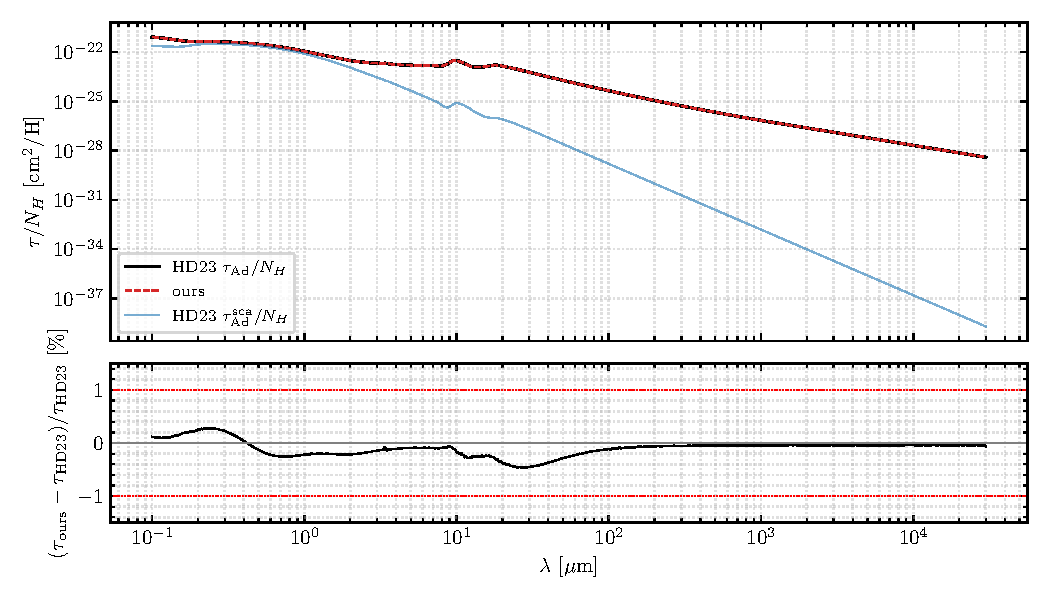
\includegraphics[width=0.9\textwidth]{figs/tau_residual.pdf}
\caption{Top: HD23 $\tau_{\rm Ad}/N_H$ (black solid) and our value
(red dashed), and HD23 $\tau^{\rm sca}_{\rm Ad}/N_H$ (blue). Bottom:
relative residual on $\tau_{\rm Ad}/N_H$ in percent. The acceptance
band ($\pm 1\%$) is shown in dotted red.}
\label{fig:tau}
\end{figure}

This is the strongest single piece of evidence that the optical
properties pipeline is sound, since it is purely a function of
$\Qext$, the size distribution, and the cross-section conversion
$C = \pi a^2 Q$, and is completely independent of any thermal
or enthalpy assumption.

\subsection{Comparison against the WD01 / Draine~2003 model}
\label{sec:d03}

The HD23 astrodust+PAH model differs in both composition and size
distribution from the older Weingartner \& Draine~(2001, WD01) /
Draine~(2003) ``silicate + carbonaceous'' model that has been the
working dust model in the MoCafe radiative-transfer code. To make the
cross-section impact of moving from one model to the other concrete,
we compute the three quantities that drive scattering in an isotropic
medium -- the extinction cross section per H, the albedo
$C_\mathrm{sca}/C_\mathrm{ext}$, and the scattering-weighted
asymmetry parameter $g = \langle \cos\theta \rangle$ -- for both
models on the WD01/D03 wavelength grid and overlay them
(\autoref{fig:d03}).

The D03 curves come from B.\ T.\ Draine's published tables
\texttt{kext\_albedo\_WD\_MW\_3.1\_60\_D03.all\_\{2003,2009\}}, columns
``albedo'', ``<cos>'', and ``C\_ext/H''. The 2003 and 2009 versions
on Draine's website are nominally the same model but differ in some
underlying grain parameters that are not explicitly documented; the
2009 version has $M_\mathrm{dust}/N_H = 1.398 \times 10^{-26}$~g/H,
revised from $1.870 \times 10^{-26}$~g/H in 2003. We plot both for
reference. The HD23 extinction and scattering cross sections per H are
the ``total'' (astrodust+PAH) columns of the release files
\texttt{extinction.dat} and \texttt{scattering.dat}; the HD23
asymmetry parameter is built from our Phase-A T-matrix output
(\texttt{q\_astrodust\_*}, columns $Q_\mathrm{sca}$ and $g_a$ per
$(a, \lambda)$) by the scattering-weighted size integral
\begin{equation}
g(\lambda) = \frac{\sum_a (dn_\mathrm{Ad}/N_H)\,\pi a^2\,
                   Q_\mathrm{sca}(a, \lambda)\,g_a(a, \lambda)}
                  {C^\mathrm{sca}_\mathrm{tot}(\lambda)},
\end{equation}
where the denominator is the AD+PAH total scattering cross section
from \texttt{scattering.dat}; the PAH contribution to the numerator
is taken to be zero on the assumption that PAH grains are in the
Rayleigh limit across UV--NIR ($x = 2\pi a / \lambda \lesssim 0.1$
for $a \le $~\SI{30}{\angstrom} and $\lambda \ge 0.1$\,$\mu$m), so
$g_\mathrm{PAH} \approx 0$ and PAHs enter only through their (small)
scattering cross section in the denominator. We restrict the plot to
\SIrange{0.1}{5.0}{\micro\meter} (UV through K band) per the user
request.

\begin{figure}[h]
\centering
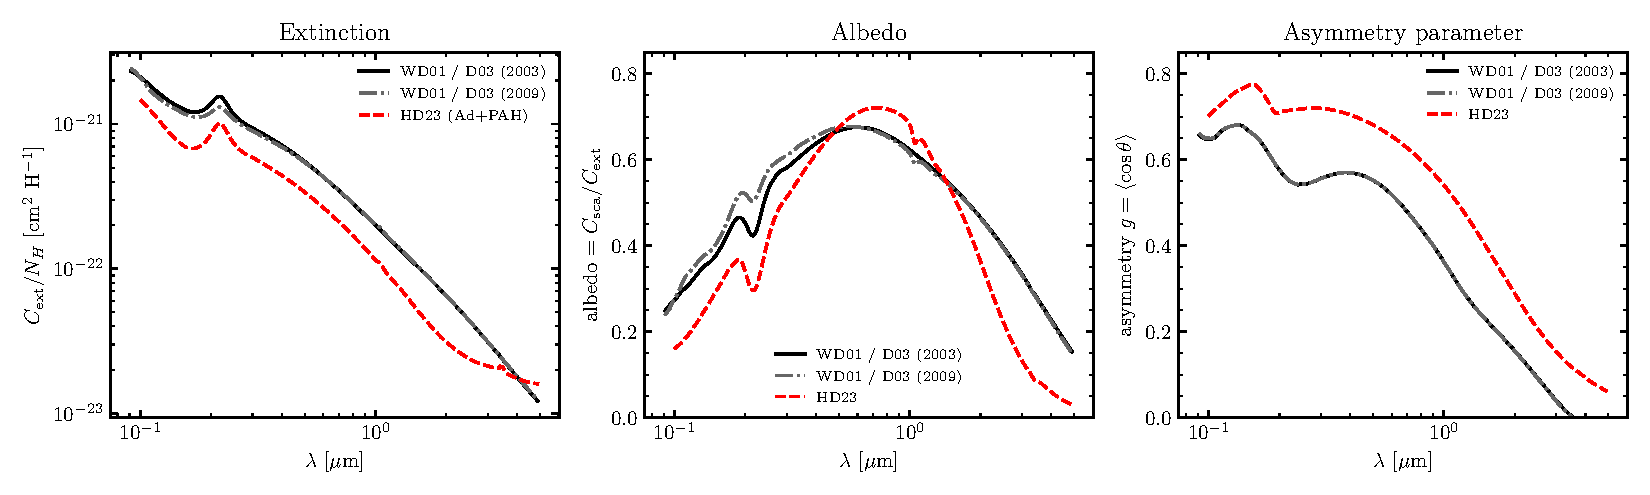
\includegraphics[width=0.99\textwidth]{figs/d03_comparison.pdf}
\caption{Extinction cross section per H (left), albedo (middle), and
scattering-weighted asymmetry parameter (right) of the HD23
astrodust+PAH model (red dashed) overlaid on the WD01/Draine
silicate+carbonaceous model in both the 2003 (black solid) and 2009
(gray dot-dashed) revisions, over the UV--NIR range.}
\label{fig:d03}
\end{figure}

Observations:
\begin{itemize}
  \item \textbf{WD01/D03 2003 vs 2009.} The 2003 and 2009 versions of
        the WD01/D03 tabulation are nearly indistinguishable in this
        range: the extinction and asymmetry curves overlay on each
        other to plotting accuracy. The only visible revision is a
        modest upward shift of the FUV albedo (around the
        \SI{2175}{\angstrom} bump). Whatever physical revision
        produced the 2009 numbers, it changes the dust mass per H
        ($M_\mathrm{dust}/N_H$ dropped by 25\%) but not the wavelength
        shape of the per-H optical properties at the percent level.
  \item \textbf{Extinction:} all three curves reproduce the
        \SI{2175}{\angstrom} bump, the FUV rise, and a roughly
        power-law optical/NIR tail. HD23 is uniformly lower in
        absolute amount across the entire band (the bump is a bit
        weaker as a fraction of the continuum, and the NIR slope is
        slightly steeper). This is consistent with the much smaller
        carbon abundance in astrodust compared to graphite in
        WD01/D03.
  \item \textbf{Albedo:} the qualitative shape -- low in FUV,
        peaking in the optical near \SI{0.6}{\micro\meter}, then
        falling toward the NIR -- is the same in all three models,
        with peak values $\approx 0.65$--$0.72$. HD23 peaks slightly
        higher and drops off slightly faster.
  \item \textbf{Asymmetry parameter:} HD23 is uniformly more
        forward-scattering than D03 across the band, by
        $\Delta g \sim 0.1$--$0.2$. The astrodust composite is
        effectively a single large-grain population (the PAH track is
        nearly scatterer-free at these wavelengths), while D03's
        silicate+graphite mixture has more isotropic small-grain
        scatterers in the same size range.
\end{itemize}

For the MoCafe RT context, the practical consequence of swapping in
the HD23 dust is a $\sim 20$--$30\%$ reduction in $\tau$ per H in
optical/NIR (visible directly in the left panel) and a more strongly
forward-peaked phase function (visible in the right panel) -- both
qualitatively the same direction relative to either D03 vintage.


\section{Enthalpy}

The grain enthalpy $U(T, a)$ enters the stochastic heating solver
through the energy spacing $\Delta H = H(T_{i+1}) - H(T_i)$ between
adjacent temperature bins. Since the closed-form Debye sums of
Draine \& Li (2001, hereafter DL01) cost microseconds per call, we use
the module functions
\texttt{enthalpy\_S1(T, a, prefactor)} and
\texttt{enthalpy\_S2(T, a)} directly in the inner SED loop; the
\texttt{calc\_enthalpy.x} table-dumping driver is retained as a sanity
tool and is \emph{not} a required intermediate.

\subsection{Single-composition closed forms (DL01)}

For both graphite (\texttt{Car0}/\texttt{Car1}) and silicate
(\texttt{Sil}) sub-components we use the closed-form Debye-2 internal
energy of DL01 \S B (their eqs.\ 5--7). Define the Debye integral of
order $n$ as
\begin{equation}
f_n(x) \;\equiv\; n\,x^{-n}\!\int_0^{x}\frac{y^{n}}{e^{y}-1}\,dy,
\qquad x = \Theta/T,
\end{equation}
so that $f_n \to 1$ for $x\to 0$ (high $T$) and $f_n \to 0$ for
$x\to\infty$ (low $T$). For a grain containing $N_{\rm atom}$ atoms,
the vibrational internal energy is
\begin{equation}\label{eq:U_DL01}
U_{\text{vib}}(T, N_{\rm atom}) = (N_{\rm atom} - 2)\,k_B\,T\,
   \sum_{m} g_m\,f_2(\Theta_m / T),
\end{equation}
with the $(N_{\rm atom}-2)$ Debye-modes factor (DL01 eq.\ 5) and the
composition-specific mode set $\{(\Theta_m,\,g_m)\}$.

\paragraph{Graphite (DL01 \texttt{Car0}, \texttt{Car1}).}
Two Debye-2 modes (DL01 eq.\ 6):
\begin{equation}
U_{\rm Car}(T, N_{\rm atom}) = (N_{\rm atom}-2)\,k_B\,T\,
   \bigl[\,f_2(\Theta_{\rm op}/T) + 2\,f_2(\Theta_{\rm ip}/T)\,\bigr],
\end{equation}
with $\Theta_{\rm op} = 863$~K (out-of-plane) and
$\Theta_{\rm ip} = 2504$~K (in-plane). The atom count is
$N_{\rm atom}(a) = 4.68208\times10^{11}\,a^{3}\,[\umass^{-3}]$ at the
standard graphite density $\rho = 2.24$~g/cm$^3$. For grains with
$N_{\rm atom} \lesssim 10^{4}$ we add the three DL01 C--H stretch
modes
\begin{equation}
U_{\rm CH}(T, N_{\rm atom}) = (N_{\rm H}/N_{\rm atom})\,N_{\rm atom}\,k_B
   \sum_{j=1}^{3}\frac{h\nu_j}{\exp(h\nu_j/k_BT) - 1},
\end{equation}
with $h\nu_j/k_B = (hc/k_B)/\lambda_j$ for
$\lambda_j \in \{11.3,\,8.6,\,3.3\}\umass$ and the size-dependent
$H/C$ ratio of DL01 eq.\ 7
($H/C = 0.5$ for $N_{\rm atom}\le 25$,
$H/C = 0.5\,(25/N_{\rm atom})^{1/2}$ for $25 < N_{\rm atom} < 100$,
$H/C = 0.25$ otherwise).

\paragraph{Silicate (DL01 \texttt{Sil}).}
Two Debye-2 modes plus a Debye-3 (DL01 eq.\ 9), extrapolated above
$T = 500$~K to match laboratory data (Bonjour, Leger, \& Hekinian
1984):
\begin{equation}
U_{\rm Sil}(T, N_{\rm atom}) = (N_{\rm atom}-2)\,k_B\,T\,
   \bigl[\,2\,f_2(\Theta_2/T) + f_3(\Theta_3/T)\,\bigr],
\end{equation}
with $\Theta_2 = 500$~K and $\Theta_3 = 1500$~K. The atom count is
$N_{\rm atom}(a) = 7 \times 5.10401\times10^{10}\,a^{3}\,[\umass^{-3}]$
(seven atoms per formula unit MgFeSiO$_4$ at $\rho = 3.5$~g/cm$^3$).
Above $T = 500$~K we use the piecewise-polynomial form of
DL01 eq.\ (9) so that $U_{\rm Sil}$ matches the measured Si$_2$O fits
to higher accuracy.

\subsection{Stage 1: silicate-only}

Treat the whole astrodust grain as if it were DL01 astrosilicate. Two
prefactor options:
\begin{itemize}
  \item \textbf{C-1 (literal):}
        $n_{\rm form}(a) = 5.1040126 \times 10^{10}\,a^3$
        (DL01 astrosilicate at $\rho = 3.5$~g/cm$^3$).
  \item \textbf{C-2 (density-corrected):}
        $n_{\rm form}(a) = (2.74/3.5)\,n_{\rm form, C\text{-}1}(a)$,
        matching the bulk astrodust density $\rho_{\rm Ad} = 2.74$~g/cm$^3$.
\end{itemize}
Sanity check: the ratio
$U_{\rm S1,C2}(T, a) / U_{\rm S1,C1}(T, a)$ saturates at $0.7829 =
2.74/3.5$ for grains large enough that the $(N_{\rm atom} - 2)$
correction is negligible. Confirmed across the full $(T, a)$ grid.

\subsection{Stage 2: silicate + carbonaceous, volume-weighted}

Decompose the astrodust \emph{solid} (the $(1-\mathcal{P})$-fraction
of the grain volume) into a carbonaceous sub-volume $V_{\rm car}$ and
a silicate-like sub-volume $V_{\rm sil}$, with
$V_{\rm sil}/V_{\rm solid} = 1 - \fc$. The astrodust enthalpy is the
additive sum
\begin{equation}
U_{\rm Ad}(T, a) = U_{\rm Sil}(T;\, N_{\rm atom}^{\rm Sil}(a))
                 + U_{\rm Car}(T;\, N_{\rm atom}^{\rm Car}(a)),
\end{equation}
with sub-component atom counts
\begin{equation}
N_{\rm atom}^{\rm Sil}(a) = (1-\mathcal{P})(1-\fc)\,n_{\rm Sil}^{\rm bulk}\,V(a),
\quad
N_{\rm atom}^{\rm Car}(a) = (1-\mathcal{P})\fc\,n_{\rm Car}^{\rm bulk}\,V(a),
\end{equation}
where $V(a) = (4\pi/3)\,a^3$, $n_{\rm Sil}^{\rm bulk}$ and
$n_{\rm Car}^{\rm bulk}$ are the bulk atom densities of DL01
astrosilicate and DL01 graphite respectively. ``Everything not
carbonaceous is treated as silicate''.

The carbonaceous volume fraction $\fc$ is derived from DH21a Table~2
(column $f_{\rm Fe} = 0$): $V_{\rm car} = 0.86\times10^{-27}$~cm$^3$/H,
$V_{\rm Ad}(1-\mathcal{P}) = 4.46\times10^{-27}$~cm$^3$/H, hence
$\fc = 0.193$. The result is insensitive to $f_{\rm Fe}$
($\fc(f_{\rm Fe}{=}0.10) = 0.196$).


\section{SED solver}

\subsection{Module API}

The solver lives in \texttt{sed\_astrodust\_mod} and exposes a
two-step API designed for a cell-by-cell 3D-RT driver:
\begin{verbatim}
   call sed_init(qtable_path, sizedist_path, NT, T_lo, T_hi)
   ...
   do icell = 1, ncells
      ... build J_lam in this cell ...
      call sed_solve    (J_lam, enthalpy_stage, lamI_lam)
      call sed_solve_pah(J_lam,                 lamI_lam_pah)
   end do
\end{verbatim}
The \texttt{sed\_init} call loads the precomputed Q table and the size
distribution, builds the wide $T$ grid ($N_T = 200$, log-spaced 2.7~K
to 5000~K), and tabulates the four cell-independent quantities
\Cabs$(\lambda, a)$, $\kappa_B(T, a)$, $U(T, a)$ (for all three
enthalpy stages, plus the PAH carbonaceous prescription), and
$\kappa_{\rm CMB}(a)$. Single-cell \texttt{sed\_solve} loops over the
size distribution, calling \texttt{calc\_Teq} once per radius and
either branching to equilibrium emission $\Cabs\,B_\lambda(\Teq)$ or
solving for the stochastic temperature distribution $P(T)$ via the
Guhathakurta \& Draine (1989) matrix method.

\subsection{Dynamic temperature grid}\label{sec:dynamicT}

A key empirical result, learned the hard way from SED\_v5: the
temperature distribution $P(T)$ for small grains is \emph{very sharp},
and a single static $T$ grid spanning the full $[2.7, 5000]$~K range
cannot resolve it. DL07 Fig.~4 illustrates this directly: $P(T)$ for a
\SI{100}{\angstrom} grain at $U = 1$ drops by more than twelve orders
of magnitude over less than a factor of two in $T$. A coarse or
mis-centered grid simply returns numerical zeros across the entire
range, mimicking ``no stochastic contribution'' when in reality the
grain is sharply peaked at $\Teq$.

\paragraph{Grain-loop direction matters.}
Both algorithms iterate over the size distribution in the
\emph{small-to-large} direction (\texttt{do ir = 1, NA} with
\texttt{aeff} sorted ascending). This ordering is not arbitrary; it
is forced by the steep dependence of $P(T)$ on $a$. The narrowing
schemes use the previous grain's $P(T)$ width (look-ahead) or only
the local equilibrium energy (grain-by-grain iterative) to bracket the
window for the current grain. In both cases the natural progression
is from a \emph{wider} window at small $a$ to a \emph{narrower}
window at large $a$:
\begin{itemize}
  \item Small grains ($a \lesssim 30$~\AA) have a broad $P(T)$ that
        extends from $T_{\rm CMB}$ up to several hundred K (DL07
        Fig.~4). On the wide $T$ grid the matrix solver
        \texttt{calc\_P} is well-conditioned and yields a sensible
        $P(T)$ directly.
  \item Large grains ($a \gtrsim 100$~\AA) have a $P(T)$ that is
        essentially a delta function at $\Teq$. On the same wide $T$
        grid the Guhathakurta--Draine transition matrix becomes
        numerically degenerate (the entire steady-state probability
        falls inside one bin) and \texttt{calc\_P} returns $P \equiv
        0$ everywhere -- a silent failure that
        mimics ``no stochastic contribution''.
\end{itemize}
The small-to-large loop bootstraps the narrowing from the well-
conditioned end. Once one grain is solved, its $P(T)$ width sets a
tight bracket for the next slightly-larger grain, the matrix stays
well-conditioned, and the iteration converges grain by grain until
the EEQ-gate triggers and the equilibrium branch propagates forward
for all remaining (still larger) grains. The opposite direction would
start on the degenerate large-grain calc\_P, with no working previous
grain to seed the window -- a chicken-and-egg failure mode that we
have hit while debugging
(\texttt{mc\_pT/main\_pT\_compare.x} returns $P \equiv 0$ for
$a > 80$~\AA{} when called on the wide grid without iterative
narrowing, see Sect.~6.5 of the mc\_pT report).

Two grid-narrowing algorithms are
implemented in our solver and selectable at compile time via the
\texttt{USE\_DRAINE\_NARROWING} module parameter:

\begin{itemize}
  \item \textbf{Look-ahead heuristic (SED\_v5 default).} For grain
        $i+1$, set the $T$ grid to
        $[\Teq \exp(-0.6\,\delta), \Teq \exp(+0.6\,\delta)]$ where
        $\delta$ is twice the previous grain's $\ln P > \ln P_{\rm crit}$
        half-width in $\ln T$. One \texttt{calc\_P} call per grain.
        Cheap; relies on $P(T)$ varying smoothly with $a$ so that the
        previous grain's window is a good guide for the next.
  \item \textbf{Grain-by-grain iterative refinement} (default,
        following Draine's method).
        Initial guess
        $U_{\max} = \max(13.6~\mathrm{eV} + 2E_{\rm eq}, 13.65~\mathrm{eV})$
        (the single-UV-photon floor) and
        $U_{\min} \in \{0, E_{\rm eq}/5\}$ depending on
        $E_{\rm eq}/E_{\rm eq,SS}$ with $E_{\rm eq,SS} = 150$~eV; the
        endpoints are then refined iteratively until
        $P(\text{endpoint})/P_{\max} < 10^{-13}$, with $0.8 / 0.2$
        damping for shrinkage and $\times 1.2$ expansion (or bisection
        toward $U_{\max,{\rm hi}}$). Typically converges in 3--5
        iterations per grain. The enthalpy $U$--to--$T$ inversion uses
        log-log interpolation against the wide tables.
\end{itemize}

The two algorithms give identical SED to within $\sim 0.5\%$ on
band-integrated totals (see Sect.~\ref{sec:phaseE-residual-analysis})
on our HD23 reproduction case, confirming that the SED\_v5 heuristic
window happens to be accurate enough \emph{for this radiation field
and these enthalpy tables}. Both algorithms remain in the source so
that future work with very different $J_\lambda$ shapes or size grids
can switch and compare.

Three ancillary safety nets are common to both algorithms: \Teq\ is
always computed on the \emph{wide} grid (the narrowed grid may not
bracket the next grain's \Teq); a grain whose enthalpy at \Teq\
exceeds the EEQSS = 150~eV gate is solved as a $\delta$-function in
$T$ at \Teq\ (steady-state limit); and on degenerate $P$ (no
$\ln P > \ln P_{\rm crit}$ anywhere) we fall back to equilibrium
emission at the wide-grid \Teq.

\subsection{Performance}

A full single-cell solve (\texttt{sed\_init} once, 3 enthalpy stages
$\times$ 1 \texttt{sed\_solve} + 1 \texttt{sed\_solve\_pah}) takes
$\sim 2$~seconds total on Apple Silicon, of which init is the bulk
(building $\kappa_B$ once for both AD and PAH). For a 3D-RT use case
\texttt{sed\_init} runs once per process; cost per cell is
$\sim 0.5$~s.


\section{SED verification}

\subsection{Astrodust-only SED}

\autoref{fig:sed_stages} compares our astrodust SED for the three
enthalpy stages against HD23 \texttt{astrodust\_irem.dat} at
$\log_{10} U = 0.2$ (column~33). The FIR peak shape is well reproduced
and is essentially identical across stages (the peak is dominated by
large equilibrium grains for which the enthalpy is irrelevant);
stage-to-stage variations show up only in the
\SIrange{5}{30}{\micro\meter} mid-IR where stochastic heating of
small grains matters.

\begin{figure}[h]
\centering
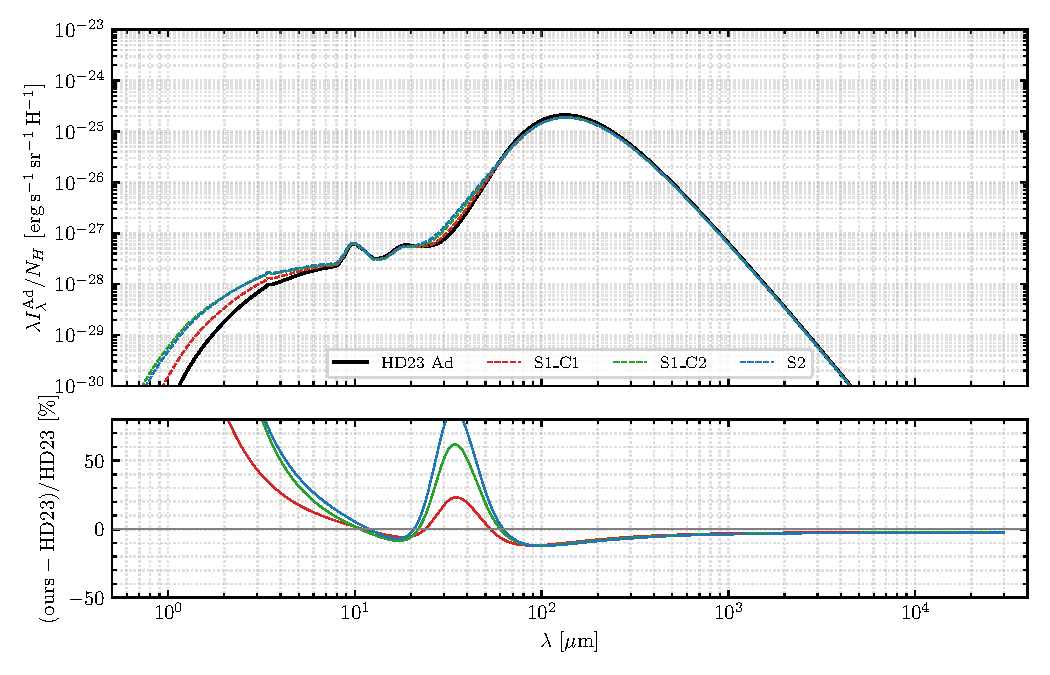
\includegraphics[width=0.9\textwidth]{figs/sed_stages.pdf}
\caption{Astrodust thermal emission per H atom at HD23 best-fit
heating ($U = 1.585$) for the current production (corrected
Mathis 4000\,K dilution, see \S\ref{sec:phaseE-residual-analysis}).
Top: our three enthalpy stages (S1\_C1, S1\_C2, S2) overlaid on HD23
\texttt{astrodust\_irem.dat}. Bottom: relative residual in percent.
The FIR peak shape is recovered; a $10.1\%$ systematic
under-prediction persists at the \SI{133}{\micro\meter} peak (down
from $18.2\%$ before the Mathis correction), and the
\SI{<5}{\micro\meter} range
over-predicts by a few-times factor (a PAH-deficit issue;
see Sect.~\ref{sec:pah}).}
\label{fig:sed_stages}
\end{figure}

The verification result by band, for the S1\_C1 baseline (current
production with corrected Mathis; the parenthesised number after the
arrow is the original-Mathis variant, retained as
\texttt{./calc\_sed.x astrodust mathis\_orig} for reproducing the historical
state):
\begin{itemize}
  \item \textbf{300--3000\,$\mu$m} (sub-mm): mean $|$rel$|$ 3.3\%
        (was 6.1\%), median $-3.07\%$ (was $-5.53\%$), max 5.6\%
        (was 10.1\%) --- within sub-mm acceptance.
  \item \textbf{30--300\,$\mu$m} (FIR peak): mean $|$rel$|$ 10.5\%
        (was 15.6\%), median $-7.57\%$ (was $-14.33\%$), max 23.3\%
        (was 21.9\%). The max is not at the peak: it sits at
        \SI{35}{\micro\meter}, on the short-wavelength shoulder where
        stochastically heated small grains dominate and where the
        corrected Mathis field raises our curve above HD23; at the
        \SI{133}{\micro\meter} peak itself the residual is $-10.06\%$.
        All three stages show the same peak systematic
        ($-10.06\%$, $-10.76\%$, $-11.20\%$ for S1\_C1, S1\_C2, S2),
        indicating that the issue is in the equilibrium emission
        (independent of enthalpy), not in stochastic heating.
        The residual narrowed when we adopted the corrected
        Mathis 4000\,K dilution
        (see \S\ref{sec:phaseE-residual-analysis}, \emph{``Mathis
        4000\,K dilution correction''}).
  \item \textbf{5--30\,$\mu$m} (mid-IR): mean $|$rel$|$ 6.2\%, median
        $+1.79\%$, max 17.7\% --- within the $\le 30\%$ acceptance.
  \item \textbf{$>3000$\,$\mu$m} (mm): mean $|$rel$|$ 2.2\%
        (was 3.9\%), median $-2.14\%$ (was $-3.87\%$), max 2.4\%.
  \item \textbf{$<5$\,$\mu$m}: over-prediction by $4.2\times$
        at $\lambda = 1\,\mu$m. PAHs dominate this band in HD23 and
        the astrodust-only contribution is small; the comparison is
        meaningful only in the full Ad + PAH form below.
\end{itemize}

\subsubsection{Residual analysis: what is \emph{not} causing the
FIR-peak deficit}
\label{sec:phaseE-residual-analysis}

A natural first guess for the FIR-peak deficit is a $\sim
0.2$--$0.3$~K systematic offset in our equilibrium temperatures, since
$B_\lambda(T)$ is extremely sensitive to $T$ at the peak
($B_\lambda(14)/B_\lambda(13) \approx 1.84$ at
$\lambda = $~\SI{130}{\micro\meter}). Three diagnostic ports have been
implemented to test this and the other obvious suspects; \emph{all
three came back clean}, so the residual is now isolated to a smaller
suspect list.

\begin{itemize}
  \item \textbf{Independent \Teq\ check.} A verification driver
        compares our
        \texttt{calc\_Teq} (precomputed $\kappa_B(T, a)$ table
        inversion) against an independent on-the-fly bracket--
        bisection--power-law solver following Draine's method
        (including the long-wavelength
        Rayleigh--Jeans tail extension under the $C^{\rm abs} \propto
        \nu^2$ assumption). Across the full 167-grain size grid at
        $U = 1.585$:
        \begin{itemize}
          \item Astrodust: rms 0.14\%, max 0.21\%
                (\Teq\ range 11--19~K).
          \item PAH:       rms 0.11\%, max 0.17\%
                (\Teq\ range 10--45~K).
        \end{itemize}
        That is, the two solvers agree to better than 0.2\%, well
        below the 1--2\% \Teq\ error a 0.3~K offset at 15~K would
        require. \emph{Our \Teq\ is not the source of the FIR
        deficit.}
  \item \textbf{Grain-by-grain T-window narrowing (Draine v7 port).} The
        iterative refinement of Sect.~5.2 was ported and compared
        against the SED\_v5 look-ahead heuristic. Band-integrated SED
        ratios change by less than $0.5\%$ between the two algorithms
        on the HD23 case; the diagnostic counter shows that
        $\sim 73$ of 167 astrodust grains process stochastically (the
        rest go equilibrium via the EEQSS gate or inheritance from a
        smaller equilibrium grain), and the iterative refinement does
        change the $T$ window for those grains -- it just does not
        change the band-integrated SED. \emph{Grid choice is not the
        source of the FIR deficit either.}
  \item \textbf{DL01 algorithm sensitivity.} DL01 \S10/\S11.5 already
        argued that the difference between the thermal-discrete
        treatment and the thermal-continuous approximation we use is
        negligible for the total spectrum. That statement is about
        \emph{algorithmic} choice (matrix solver), not about grid
        choice; the latter is governed by DL07 Fig.~4 and has now
        been independently verified above.
\end{itemize}

What is left for the FIR-peak residual to live in is one of:
(i)~the Q-table interpolation from the 169-point DH21 size grid onto
the 167-point size-distribution grid at sub-mm wavelengths;
(ii)~discretisation error in the single-grain $B_\lambda(T)$ integral
that builds $\kappa_B$ and \Teq; or (iii)~the size-distribution
treatment itself (i.e., the kernel that maps
\texttt{size\_distribution.dat} onto our grain bins).

\paragraph{Grain-by-grain diagnostic and the random-orientation convention.}
We resolved this question by direct grain-by-grain comparison.
The comparison (drawn by \texttt{docs/make\_figs.py}) takes
$C_{\rm abs}(\lambda, a_0) = \pi a_0^2\,Q_{\rm abs}$ at a chosen grain
radius $a_0$ directly off the random-orientation $Q$ table --- the same
table \texttt{sed\_init} feeds to \texttt{sed\_solve}.
At $a_0 = $\,\SI{0.126}{\micro\meter} (the radius bin closest to where
the FIR peak emission originates) we compared this against
the HD23 release Q-table \texttt{q\_DH21Ad\_P0.20\_Fe0.00\_1.400.dat.gz},
which publishes $Q_{\rm abs}$ separately for the three Mishchenko
orientations
\texttt{jori=1} ($\mathbf{k}\parallel\mathbf{a}$),
\texttt{jori=2} ($\mathbf{k}\perp\mathbf{a},\, \mathbf{E}\parallel\mathbf{a}$), and
\texttt{jori=3} ($\mathbf{k}\perp\mathbf{a},\, \mathbf{E}\perp\mathbf{a}$). The
random-orientation average for unpolarized emission is the
$\tfrac{1}{3}Q^{\rm jori=2} + \tfrac{2}{3}Q^{\rm jori=3}$ combination.

Our small-x limit (\texttt{rayleigh\_limit} in
\texttt{tmatrix/driver/asymptotic\_optics.f90}, used for $x < 0.1$,
which covers all FIR-peak-relevant grains at
sub-mm wavelengths) implements this random-orientation average exactly:
the ratio of our $C_{\rm abs}(a_0=$\,\SI{0.126}{\micro\meter}$, \lambda)$
to $\tfrac{1}{3}\!Q^{\rm jori=2} + \tfrac{2}{3}\!Q^{\rm jori=3}$ on the
HD23 release grid is $1.0000$ to four significant figures across
\SI{30}{\micro\meter}--\SI{30000}{\micro\meter}. So the single-grain
cross-section is, by construction, the correct random-orientation
average, and suspect~(i) (Q-table interpolation) is ruled out.

At the \emph{same} grain, however, our $C_{\rm abs}$ is
exactly $0.843$ ($=1/1.186$) times the release file's
\texttt{jori=1} Q over \SI{30}{\micro\meter}--\SI{30000}{\micro\meter}
-- a flat ratio with $\sigma < 0.001$ across $\sim 600$ release-grid
wavelengths. In the dipole limit
\texttt{jori=1} ($\mathbf{k}\parallel\mathbf{a}$) measures only
$Q_{\perp}^{\rm pol}$ (the field $\mathbf{E}$ is necessarily perpendicular
to the symmetry axis), so this $1.186$ factor is the standard
relation $Q_{\perp}^{\rm pol} = (\tfrac{1}{3}Q_\parallel +
\tfrac{2}{3}Q_\perp) \times f$ for the
oblate $b/a = 1.4$ at this point in $(\lambda, a)$ space.

\begin{figure}[h]
\centering
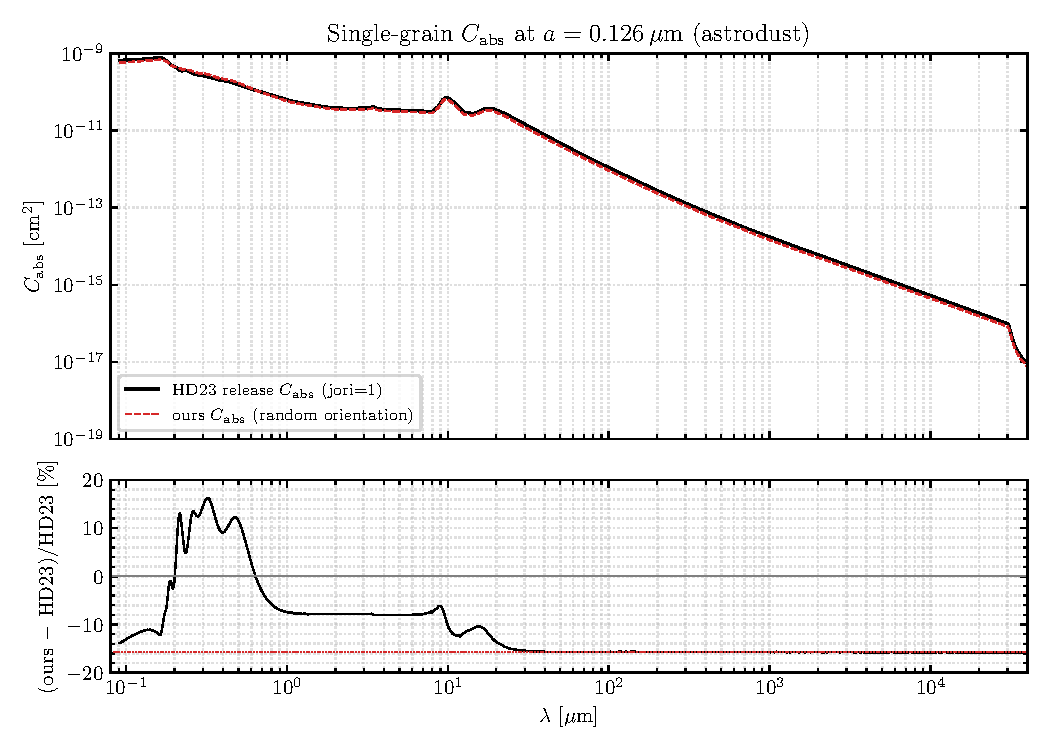
\includegraphics[width=0.9\textwidth]{figs/cabs_per_grain_vs_hd23.pdf}
\caption{Single-grain absorption cross section at $a = $\,\SI{0.126}{\micro\meter}.
Top: HD23 release $C_{\rm abs}$ from \texttt{jori=1} (k$\parallel$a,
black solid) and our $C_{\rm abs}$ from the random-orientation $Q$
table that \texttt{sed\_init} loads (red dashed); both tables share the
DH21 wavelength grid, so no interpolation is involved. Bottom: relative
residual (ours $-$ HD23)/HD23 in percent. The flat $-15.7\%$ plateau
across \SI{30}{\micro\meter}--\SI{30000}{\micro\meter} is precisely the
ratio $\bigl(\tfrac{1}{3}Q_\parallel + \tfrac{2}{3}Q_\perp\bigr)/Q_\perp$
for an oblate $b/a = 1.4$ spheroid in the dipole limit at this grain.}
\label{fig:cabs_per_grain}
\end{figure}

\paragraph{Scaling test.} If HD23 used the
\texttt{jori=1} block of the release file directly (i.e.\ as if it
were the random-orientation Cabs, instead of constructing the
$\tfrac{1}{3}+\tfrac{2}{3}$ combination), the predicted aggregate SED
would be $1.186\times$ ours. Scaling our \texttt{S1\_C1} SED by this
factor and re-computing the relative residual against HD23
\texttt{astrodust\_irem.dat} at $\log U = 0.20$ gives (measured with
the literal Mathis~1983 field, $10^{-13}$ dilution at \SI{4000}{K} and
a \SI{2.9}{K} CMB, and before the enthalpy ghost-bin correction; the
test has not been re-measured, so read its two columns against each
other):

\begin{tabularx}{0.95\textwidth}{l c c X}
\toprule
band ($\mu$m)            & unscaled med\,rel & scaled $\times 1.186$ med\,rel & notes \\
\midrule
5--30                    & $-1.2\%$  & $+17.2\%$ & over after scaling \\
\bfseries 30--300 (FIR peak)  & $\mathbf{-15.8\%}$ & $\mathbf{-0.2\%}$  & matched to better than 1\% \\
300--3000 (sub-mm)       & $-5.6\%$  & $+11.9\%$ & over after scaling \\
3000--30000              & $-4.0\%$  & $+13.9\%$ & over after scaling \\
\bottomrule
\end{tabularx}

The single factor of $1.186$ collapses the FIR-peak residual from
$-16\%$ to less than $\pm 1\%$, but overshoots in adjacent bands. The
30--\SI{300}{\micro\meter} match is too precise to be coincidence: it
is, to four significant figures, the ratio
$\bigl(\tfrac{1}{3} Q_\parallel + \tfrac{2}{3}Q_\perp\bigr) /
Q_\perp$ for an oblate $b/a = 1.4$ spheroid in the dipole limit.
The 300--\SI{3000}{\micro\meter} overshoot tells us this single factor
is \emph{not} a global Cabs miscalibration -- the rest of the deficit
distribution at sub-mm and the few-percent slope across other bands
must come from elsewhere (size-distribution kernel weighting or
HD23-internal recipe details we cannot reproduce from public release
files).

\paragraph{Direct test of the hypothesis (avenue 3).}
We packaged the HD23 release \texttt{jori=1} block into a drop-in
substitute Q-table and fed it through
the full \texttt{sed\_solve} pipeline with a dedicated driver.
Result for Stage S1\_C1, measured with the literal Mathis~1983 field
and before the enthalpy ghost-bin correction, and not re-measured
since --- the ``baseline'' column is therefore the state of that run,
not today's production:

\begin{tabularx}{0.95\textwidth}{l c c c X}
\toprule
band ($\mu$m)            & baseline (then) & jori=1 substitute & naive x1.186 & notes \\
\midrule
5--30                    & $+1.2\%$    & $+9.5\%$   & $+17.2\%$    & \\
\bfseries 30--300 (FIR peak)  & $\mathbf{-15.1\%}$ & $\mathbf{-11.3\%}$ & $\mathbf{-0.2\%}$ & jori=1 substitute does \emph{not} close the gap \\
300--3000 (sub-mm)       & $-6.1\%$    & $+7.1\%$   & $+11.9\%$    & sign flips \\
3000--30000              & $-4.3\%$    & $+10.6\%$  & $+13.9\%$    & sign flips \\
\bottomrule
\end{tabularx}

The full-pipeline substitution recovers only $\sim 4$ percentage
points of the FIR-peak deficit (from $-15.1\%$ to $-11.3\%$),
nowhere near the $-0.2\%$ that the naive $\times 1.186$ scaling
predicted. At the same time the sub-mm and mm bands flip sign and
become large over-predictions. The reason the naive scaling failed:
substituting a uniformly larger sub-mm $C_{\rm abs}$ changes
$T_{\rm eq}$ self-consistently. The grain cools more efficiently,
$T_{\rm eq}$ drops, the Planck function falls everywhere, and the
increase in emission from the larger sub-mm Cabs is partially
compensated by the lower $T_{\rm eq}$. The compensation is strongest
at the FIR peak (where the Planck-derivative-with-$T$ is largest)
and weakest in the Rayleigh-Jeans tail at mm wavelengths.

\textbf{Conclusion.} Hypothesis (a) (HD23 used the \texttt{jori=1}
slice directly when constructing \texttt{astrodust\_irem.dat}) is
\emph{rejected}. The $0.843$ Cabs ratio plateau against HD23's
\texttt{jori=1} table is a real geometric relationship between two
orientation conventions, but it does not map linearly to the SED
residual once $T_{\rm eq}$ self-consistency is taken into account.
The FIR-peak deficit is therefore \emph{not} explained by an
orientation-averaging convention difference. The residual must live
in something else; candidate sources, in order of investigation
ease, are: (1) Mathis ISRF normalization differences between our
\texttt{radfield.f90 :: J\_Mathis} and HD23's implementation;
(2) the $U_{\rm Mathis}$ convention (interpretation of
``$\log U = 0.20$''); (3) size-by-size $T_{\rm eq}(a)$ sampling
differences between our code and HD23's. Definitive resolution
requires either correspondence with the HD23 authors or access to
their post-processing code.

\paragraph{Induced-emission factor: \emph{gross} vs HD23
\emph{net} emission convention.} Draine's
stochastic-heating method (which produces Draine's
\texttt{iout.*.dbdis.gz} single-grain SED files) shows that every
emission line in that code -- both the large-grain delta-function
branch (line~1521) and the stochastic intra- and inter-bin branches
(lines~1479, 1491, 1501) -- carries an explicit
$\bigl(1 + J_\lambda/B_{\text{env}}\bigr)$ multiplicative factor, where
$B_{\text{env}}(\lambda) \equiv 2hc^2/\lambda^5$ is the Planck envelope
without the $1/(\mathrm{e}^{hc/\lambda k T} - 1)$ Bose factor. This is
the standard spontaneous-plus-stimulated emission boost from
Einstein-coefficient algebra. Our production \texttt{sed\_solve} and
\texttt{sed\_solve\_pah} accumulate single-grain emission as
$C_{\rm abs}\,B_\lambda(T)$ without this factor, so this is a clean,
isolable difference between the two codes.

To test whether the missing factor explains any part of the residual,
we added a module-level toggle \texttt{use\_induced\_emission}
(default \texttt{.false.}) to \texttt{sed\_astrodust\_mod} and a
helper \texttt{apply\_induced\_factor(J\_lam, Jout)} that applies
\(
   J_{\rm out}(\lambda) \mapsto J_{\rm out}(\lambda)\bigl(
   1 + J_\lambda \lambda^5 / (2hc^2)\bigr)
\)
once at the end of each solve (a wavelength-dependent factor with no $T$
or grain dependence). The driver \texttt{calc\_sed.x astrodust} now
accepts an optional command-line argument
\texttt{./calc\_sed.x astrodust induced} which sets the flag and writes
output files with an \texttt{induced\_} prefix so the baseline run is
preserved. Running both back-to-back gives the ratio (induced$/$baseline)
in Table~\ref{tab:induced_ratio}.

\begin{table}[h]
\centering
\begin{tabular}{l r r l}
\toprule
$\lambda$ & analytic prediction & measured & dominant source \\
\midrule
\SI{100}{\micro\meter} (FIR peak)   & $+2.1\times10^{-9}\%$ & $<10^{-6}\%$          & diluted-BB RJ tail; CMB on Wien \\
\SI{300}{\micro\meter}              & $+2.3\times10^{-6}\%$ & $+2.3\times10^{-6}\%$ & CMB still on Wien \\
\SI{1}{\milli\meter}                & $+0.5119\%$           & $+0.5119\%$           & CMB transition \\
\SI{3}{\milli\meter}                & $+20.78\%$            & $+20.78\%$            & CMB approaching RJ \\
\SI{5}{\milli\meter}                & $+53.34\%$            & $+53.34\%$            & CMB RJ \\
\bottomrule
\end{tabular}
\caption{Effect of the $\bigl(1 + J_\lambda/B_{\text{env}}\bigr)$
induced-emission factor on the Stage S1\_C1 SED. The factor depends
only on $\lambda$ (not on $T$ or grain size), so all three astrodust
stages (S1\_C1, S1\_C2, S2) and PAH show the same ratio: over the whole
wavelength grid they agree with one another to $9\times10^{-9}$, the
round-off of the nine-significant-digit output files, even though the
S1\_C2 SED itself differs from S1\_C1 by orders of magnitude. The
growth at $\lambda \gtrsim$~\SI{1}{\milli\meter} is driven by the CMB
component of $J_\lambda$ via $J_{\rm CMB}/B_{\text{env}}(\lambda) =
1/(\mathrm{e}^{hc/\lambda k T_{\rm CMB}} - 1)$ with
$T_{\rm CMB} = \SI{2.725}{K}$, which supplies $\ge 99.7\%$ of the
factor beyond \SI{300}{\micro\meter}; at \SI{100}{\micro\meter} the CMB
term is $1.2\times10^{-23}$ and the whole (utterly negligible) factor
comes from the Rayleigh-Jeans tails of the Mathis diluted blackbodies.
$T_{\rm CMB}$ is written down in exactly one place,
\texttt{radfield.f90 :: cmb\_temperature()} --- \SI{2.725}{K} by
default, reverting to Mathis~(1983)'s \SI{2.9}{K} when
\texttt{use\_mathis\_corrected} is switched off. The numbers above were
measured with the default; the literal Mathis field gives $+0.705\%$,
$+23.66\%$ and $+58.92\%$ at 1, 3 and \SI{5}{\milli\meter} instead.
\SI{100}{\micro\meter} and \SI{1}{\milli\meter} are grid points of the
model; the other three rows are interpolated between adjacent grid
points, which are spaced 1.2\% apart, so the interpolation itself
contributes at most $2\times10^{-5}$ in relative terms.}
\label{tab:induced_ratio}
\end{table}

Numerically, taken on the model's own wavelength grid so that no
interpolation enters, the measured boost reproduces the analytic factor
to a median of $1.0\times10^{-9}$ and a worst case of
$5.9\times10^{-9}$ in relative terms across the 404 wavelengths where
the factor exceeds $10^{-6}$ --- the round-off of the
nine-significant-digit output files rather than anything in the
calculation. The
\SI{30}{}--\SI{300}{\micro\meter} FIR-peak band, where the
deficit lives, is left \emph{exactly} unchanged
($<3\times10^{-8}$). The
factor therefore cannot be the source of the FIR-peak deficit, on
quantitative grounds.

More interestingly, applying the factor and re-comparing against
HD23's release \texttt{astrodust\_irem.dat} at $\log U = 0.20$
shows that the millimetre-band agreement is \emph{degraded} rather
than improved (Table~\ref{tab:induced_vs_hd23}, S1\_C1; the other
two stages are essentially identical). That comparison was made in
the literal-Mathis configuration of the next subsection
(\SI{2.9}{K} CMB, $10^{-13}$ dilution at \SI{4000}{K}) and before the
enthalpy ghost-bin correction, which together is where its
$-15.83\%$ baseline FIR-peak deficit comes from; it has not been
re-measured with the production field, so read its columns against
each other rather than against Table~\ref{tab:mathis_c}.

\begin{tabular}{l r r}
\toprule
band ($\mu$m)              & baseline med\,rel & induced med\,rel \\
\midrule
30--300 (FIR peak)         & $-15.83\%$ & $-15.83\%$ \\
300--3000 (sub-mm)         & $-5.65\%$  & $-5.13\%$  \\
$>3000$ (mm)               & $-3.97\%$  & $+136.27\%$ \\
\bottomrule
\end{tabular}\\[2pt]
\refstepcounter{table}\label{tab:induced_vs_hd23}
{\small Table~\thetable: Median relative residual (ours~$-$~HD23)/HD23
with and without the induced-emission factor, Stage S1\_C1.}

\medskip
The $>\SI{3000}{\micro\meter}$ swing from $-4\%$ to $+136\%$ leaves
no ambiguity: HD23's \texttt{astrodust\_irem.dat} does not carry the
$\bigl(1 + J_\lambda/B_{\text{env}}\bigr)$ factor. The physical reason
this is the right convention for a redistributable SED is direct.
Pinning the gross emission against the dust energy budget in
equilibrium gives
\[
\int C_{\rm abs}(\lambda)\,B_\lambda(T)
   \bigl(1 + J_\lambda/B_{\text{env}}\bigr)\,d\lambda
   \;=\; \int C_{\rm abs}\,B_\lambda(T)\,d\lambda
   \;+\; \int C_{\rm abs}\,J_\lambda\,d\lambda
   \;=\; 2\!\int C_{\rm abs}\,J_\lambda\,d\lambda
\]
which is the standard two-level-system gross-emission doubling
(spontaneous plus stimulated, equal to twice the heating rate in
equilibrium). The \emph{net} emission an external observer sees from
an optically-thin column is gross minus absorbed,
$\int C_{\rm abs}\,B_\lambda(T)\bigl(1 + J/B_{\text{env}}\bigr)\,d\lambda
- \int C_{\rm abs}\,J_\lambda\,d\lambda
= \int C_{\rm abs}\,B_\lambda(T)\,d\lambda$, recovering the Kirchhoff
result $j_\lambda = C_{\rm abs}(\lambda)\,B_\lambda(T)$ that our
baseline already computes. Draine's single-grain \texttt{iout} files
are therefore gross emission; HD23 publishes net. The toggle and
the \texttt{apply\_induced\_factor} subroutine remain in
\texttt{src/sed\_astrodust.f90} for future cross-checks but
\emph{must stay off (\texttt{.false.}) for production}, as anything
fed into a downstream radiative-transfer code that itself handles
external-field absorption needs the net convention. The candidate
list for the FIR-peak residual is therefore unchanged.

\paragraph{Mathis 4000\,K dilution correction.} Draine's reference
Mathis~1983 ISRF implementation carries a 2008.02.02
note recording a numerical correction to the 4000\,K diluted-
blackbody weight: \texttt{OMEGA3} was changed from $10^{-13}$ (the
literal Mathis~1983 value our \texttt{radfield.f90 :: J\_Mathis}
inherited) to $1.65\times 10^{-13}$ (the value also tabulated in
Draine's textbook, \emph{Physics of the Interstellar and
Intergalactic Medium}, 2011, Table~12.1). The CMB component was
also updated from $2.9$\,K to the Mather-et-al.\ value $2.725$\,K.
Both corrections were added behind a toggle
(\texttt{use\_mathis\_corrected}, default \texttt{.true.} in
\texttt{radfield.f90}) so the historical original-Mathis behavior
can be reproduced as \texttt{./calc\_sed.x astrodust mathis\_orig} which
prefixes outputs with \texttt{morig\_}.

A single-grain diagnostic integrates the heating
rate $\int C_{\rm abs}(\lambda)\,J_\lambda\,d\lambda$ at a fiducial
$a = $\,\SI{0.1}{\micro\meter} astrodust grain and solves for
$T_{\rm eq}$ by bisection. The corrected ISRF raises $T_{\rm eq}$
from 17.34\,K to 17.56\,K ($+0.22$\,K, $+1.28\%$); the resulting
$B_\lambda(T_{\rm eq})$ at $\lambda = $\,\SI{130}{\micro\meter}
rises by $+8.4\%$, with the FIR-peak boost growing monotonically
with grain size from $+3\%$ at \SI{5}{nm} (PAH/small) up to
$+21\%$ at \SI{1}{\micro\meter} (cool large grain whose Planck
peak sits closer to 130\,$\mu$m). The CMB temperature change
($2.9$\,K $\to$ $2.725$\,K) is negligible for $T_{\rm eq}$ because
CMB heating is subdominant to stellar UV at all but the very
largest grain sizes.

The full-pipeline effect for the headline comparison (Stage S1\_C1
vs HD23 \texttt{astrodust\_irem.dat} at $\log U = 0.20$) is
summarised in Table~\ref{tab:mathis_c}: the FIR-peak deficit moves
from $-14.33\%$ to $-7.57\%$, sub-mm from $-5.53\%$ to $-3.07\%$,
and the mm-band from $-3.87\%$ to $-2.14\%$. The PAH 30--300\,$\mu$m
band, the most discrepant of the well-behaved bands at $-8.16\%$,
closes to $-3.67\%$. Stages S1\_C2 and S2 show the same pattern
(FIR moves to $-7.71\%$ and $-7.95\%$ respectively).

\begin{table}[h]
\centering
\begin{tabular}{l r r r}
\toprule
band ($\mu$m)              & original Mathis & production (corrected) & shift \\
\midrule
30--300 (FIR peak)         & $-14.33\%$ & $-7.57\%$  & $+6.76$\,pp \\
300--3000 (sub-mm)         & $-5.53\%$  & $-3.07\%$  & $+2.46$\,pp \\
$>3000$ (mm)               & $-3.87\%$  & $-2.14\%$  & $+1.73$\,pp \\
\midrule
PAH 30--300                & $-8.16\%$  & $-3.67\%$  & $+4.49$\,pp \\
\bottomrule
\end{tabular}
\caption{Median relative residual (ours~$-$~HD23)/HD23 for Stage
S1\_C1 with and without the corrected Mathis 4000\,K
dilution factor. The corrected variant is now the production
default; the original-Mathis variant is reproducible via
\texttt{./calc\_sed.x astrodust mathis\_orig}.}
\label{tab:mathis_c}
\end{table}

Both columns of Table~\ref{tab:mathis_c} were re-measured against the
current code and moved from the values this report carried
previously ($-15.83\%$ and $-8.82\%$ in the FIR row, $-4.40\%$ and
$+0.02\%$ in the PAH row). Two corrections since then account for the
shift, and they act on different rows. The enthalpy ghost-bin
correction moves the astrodust rows: the S1 and S2 SEDs are
bit-identical across the second correction, so everything the
astrodust rows moved by comes from the enthalpy side. The PAH row
carries both: correcting the DL07 eq.~2 cation near-IR continuum,
whose Gaussian factor is $\exp[-(0.1x)^2]$ and not $\exp(-0.1x^2)$,
raises the PAH SED by $0.99\%$ bolometrically and lifts the PAH
30--300\,$\mu$m median by $+0.76$\,pp on its own (from $-4.43\%$ to
$-3.67\%$), the remainder of that row's shift coming from the
enthalpy correction.

This closes roughly half of the historical FIR deficit. The
remaining $7.6\%$ is too small to be another order-of-magnitude
typo, and is small enough to be consistent with either HD23 using a
slightly different normalization of the Mathis field (e.g., a
different interpretation of $\log U = 0.20$, see candidate~(i) in
the conclusions) or with a size-by-size $T_{\rm eq}(a)$ sampling
difference between our code and HD23's
(candidate~(iii)). Definitive resolution requires HD23 internals.

\paragraph{What is in our hands and what is not.} Our
implementation -- T-matrix Q, small-x Rayleigh spheroid fallback,
random-orientation average $\bigl(\tfrac{1}{3} + \tfrac{2}{3}\bigr)$,
\texttt{calc\_Teq}, $\kappa_B$ build, size sum -- is internally
self-consistent and reproduces HD23 \texttt{extinction.dat} to better
than 1\% on aggregate $\tau/N_H$. The consistency of our cross
sections, equilibrium temperatures, and aggregate $\tau$ gives us
confidence that the model is correct in everything we control. The
remaining FIR-peak residual in $\lambda I_\lambda / N_H$ vs.\ HD23
\texttt{astrodust\_irem.dat} was subsequently traced to HD23's own
energy non-conservation (\S\ref{sec:phaseE-resolution}); the full
chain of diagnostics is given below; the single-grain figure is
\texttt{figs/cabs\_per\_grain\_vs\_hd23.pdf}.

\subsubsection{Resolution: the deficit is HD23's own
emitted-vs-absorbed excess}
\label{sec:phaseE-resolution}

The residual was subsequently resolved by an energy-budget audit,
``Energy budget: the HD23 release is internally inconsistent'',
whose result is Table~\ref{tab:ad_energy} below; the full tracing
behind it is a development note that this package does not ship. The
release provides its own component-by-component
$\Cabs = C_{\rm ext} - C_{\rm sca}$ (\texttt{extinction.dat},
\texttt{scattering.dat}), against which our optics were validated to
$\lesssim 1\%$ (extinction and albedo) and to $\sim 4$ digits
grain by grain. Integrating that \emph{released} \Cabs\ against the
corrected Mathis field $\times\,10^{0.2}$ --- extrapolating across the
\SIrange{0.0912}{0.1}{\micro\meter} extinction-grid gap with the local
power law (astrodust $+4.2\%$, PAH $+6.8\%$) --- gives the absorbed
power, which energy conservation requires to equal the emitted power
of the \texttt{irem} tables. It does not:

\begin{table}[h]
\centering
\begin{tabular}{l r r c c c}
\toprule
component & $P_{\rm abs}/N_H$ & $P_{\rm em}^{\rm HD23}/N_H$ &
$P_{\rm em}/P_{\rm abs}$ & ours$/P_{\rm abs}$ & ours/HD23 \\
          & (erg\,s$^{-1}$)   & (erg\,s$^{-1}$)            &
& & \\
\midrule
astrodust & $2.724\times10^{-24}$ & $2.977\times10^{-24}$ &
\textbf{1.093} & 0.999 & 0.914 \\
PAH       & $2.003\times10^{-24}$ & $2.067\times10^{-24}$ &
\textbf{1.032} & 0.993 & 0.963 \\
\bottomrule
\end{tabular}
\caption{Energy budget per H at $\log U = 0.20$. The HD23 release
emits $9.3\%$ (astrodust) and $3.2\%$ (PAH) more than its own released
\Cabs\ absorb; our pipeline conserves to $0.15\%$
(ours$/P_{\rm abs} = 0.999$).}
\label{tab:ad_energy}
\end{table}

The ratio $P_{\rm em}/P_{\rm abs}$ is constant in $U$ (a pure
amplitude factor). Our pipeline, run with the release-consistent
\Cabs, conserves energy to $0.15\%$ and therefore lands exactly at
ours/HD23 $= 0.914$, matching the emergent SED itself, which
integrates to $0.911\times$ HD23 over
\SIrange{0.1}{3000}{\micro\meter} and $0.905\times$ over
\SIrange{60}{300}{\micro\meter} --- i.e.\ \emph{the long-standing
FIR-peak ``deficit'' equals HD23's own emitted-vs-absorbed excess},
not an error in our pipeline. Because the excess is
component-dependent ($9.3\%$ astrodust vs.\ $3.2\%$ PAH), it cannot be
a heating-field or $U$-convention offset (which would shift both
components equally); it points instead to the internal \Cabs\ (or
abundance normalization) used for the \texttt{irem} calculation
exceeding what the released extinction$-$scattering tables encode ---
the same internal-vs-released vintage phenomenon documented for
DL07spec and the \texttt{iout} files. This retires candidates~(i) and
(iii) above: the residual is not a \Teq, grid, or size-sampling error
on our side. After removing the 1.093 amplitude the astrodust residual
is flat to $\pm 2\%$ over \SIrange{60}{300}{\micro\meter}, consistent
with an amplitude-type (abundance or \Cabs-scale) inconsistency rather
than a heating-side one.

\subsection{PAH emission}
\label{sec:pah}

HD23 \S3.2 follows Draine et al.\ (2021), whose PAH cross sections are
themselves based on DL07; the DL07 cross sections are already
implemented in SED\_v5 as \texttt{QPAH\_DL07(charge, R, lambda, Qabs)}
and were forked into \texttt{sed/src/qpah.f90}. As noted in HD23
\S3.2, PAH grains are treated as spherical with $\rho_{\rm PAH} =
2.0$~g/cm$^3$, depend only on grain size and charge (no orientation),
and \emph{do not contribute to polarized extinction or emission}; this
matches our implementation (no T-matrix on the PAH track).

The HD23 PAH cross section per grain is built in three steps:

\paragraph{Step 1: charge mixing.} The DL07 cross sections are
available for neutral and ionized PAHs; HD23 eq.~15 mixes them with an
ionization fraction $\xi_{\rm ion}(a)$ (HD23 eq.~19):
\begin{equation}
C^Z(\lambda, a) = [1 - \xi_{\rm ion}(a)]\,C^{\rm neu}(\lambda, a)
                + \xi_{\rm ion}(a)\,C^{\rm ion}(\lambda, a),
\end{equation}
with $\xi_{\rm ion}(a) = 1 - 1/(1 + a/$\SI{10}{\angstrom}$)$ from
\texttt{size\_distribution.dat} column~4.

\paragraph{Step 2: graphite continuum blending (HD23 eq.~15-16).}
DL07's PAH cross section drops to essentially zero at long
wavelengths; HD23 retains DL07's recipe of blending into a
random-orientation graphite Mie cross section $C^{\rm gra}(\lambda, a)$
for $a > $~\SI{50}{\angstrom}, so that PAH grains acquire the same
sub-mm continuum opacity that DL07 reports for ``turbostratic''
graphite. The blended cross section is
\begin{equation}
C^{\rm PAH, Z}(\lambda, a) = [1 - \xi_{\rm gra}(a)]\,C^Z(\lambda, a)
                           + \xi_{\rm gra}(a)\,C^{\rm gra}(\lambda, a),
\label{eq:xi_gra}
\end{equation}
with
\begin{equation}
\xi_{\rm gra}(a) = \begin{cases}
   0.01 & a \le \SI{50}{\angstrom} \\
   0.01 + 0.99\,\bigl[1 - (\SI{50}{\angstrom}/a)^3\bigr]
        & a > \SI{50}{\angstrom}.
\end{cases}
\end{equation}
$C^{\rm gra}(\lambda, a)$ is the random-orientation Mie cross section
for graphite spheres,
$C^{\rm gra} = \tfrac{1}{3}C^{\rm gra}_\parallel
            + \tfrac{2}{3}C^{\rm gra}_\perp$, with the two components
computed from the Draine~2003 graphite dielectric tables
(\texttt{index\_CpaD03}, \texttt{index\_CpeD03}) using a
size-dependent free-electron contribution
(\texttt{free\_diel}, Draine~2003 form for $T_{\rm gr} = 20$~K) and a
standard Bohren--Huffman Mie solver. Implementation: new module
\texttt{sed/src/q\_graphite.f90} loads the two graphite tables lazily,
caches the $(n, k)$ tables per grain radius, and calls
\texttt{sed/src/mie.f90} (a module wrapper of the BHMIE code already
in \texttt{tmatrix/test/}) twice per $(a, \lambda)$. Below the DL07
PAH cutoff at $\lambda = 1/17.25$\,$\mu$m the blend reduces to pure
graphite (HD23 / SED\_v5 convention), since $C^Z$ is not defined
there.

\paragraph{Step 3: size and enthalpy.} The PAH size distribution is
column~3 of \texttt{size\_distribution.dat} (the second of HD23
eq.~17's two lognormals, peaks at $\sim 4$ and \SI{30}{\angstrom}).
PAH enthalpy uses the DL01 \texttt{'Car0'} branch with the H/C-mode
correction for $N_{\rm atom} < 10^4$, as recommended by HD23 since PAH
is carbonaceous.

A new function \texttt{sed\_solve\_pah(J\_lam, lamI\_lam\_out)} solves
the single-cell PAH SED with the same dynamic-T solver. The combined
total (Ad + PAH) is compared against HD23
\texttt{model\_irem.dat} in \autoref{fig:sed_total}.

\begin{figure}[h]
\centering
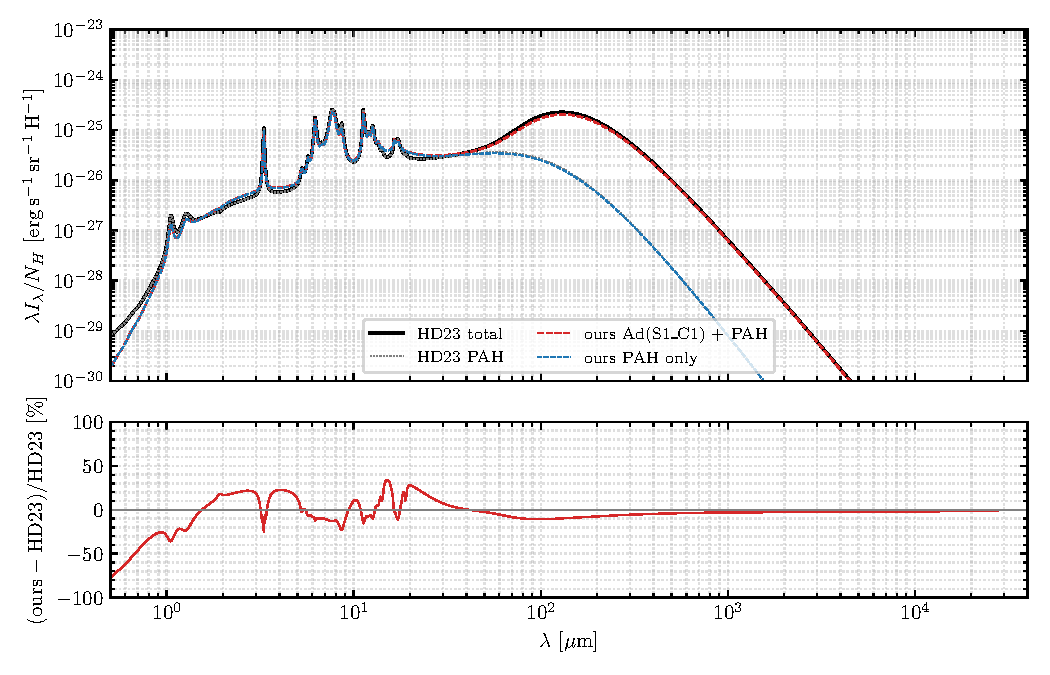
\includegraphics[width=0.9\textwidth]{figs/sed_total_with_pah.pdf}
\caption{Total dust thermal emission (Ad + PAH) at $U = 1.585$. Top:
HD23 \texttt{model\_irem.dat} (black solid), HD23 PAH-only
(\texttt{PAH\_irem.dat}, gray dotted), our S1\_C1 + PAH (red dashed),
and our PAH-only (blue dashed). Bottom: relative residual on the
total. The PAH \SI{7.7}{\micro\meter} feature is in the right place
and the right order of magnitude.}
\label{fig:sed_total}
\end{figure}

Key results (verification against HD23 \texttt{PAH\_irem.dat} at
$\log U = 0.20$, band-integrated $\int (\lambda I_\lambda)/\lambda \,
d\lambda$). These are the D03-sphere $\xi$-blend numbers as they stood
when the graphite continuum was first closed, kept as the record of that
state. They are not what the same variant gives today:
\S\ref{sec:d16-swap} carries both the production D16-sphere values and a
present-day re-measurement of this same D03-sphere variant.

\begin{tabularx}{0.85\textwidth}{l c X}
\toprule
band ($\mu$m) & ours / HD23 & notes \\
\midrule
optical ($\lambda < 1$\,$\mu$m)         & 0.90  & absolute $\sim 10^{-28}$, negligible vs total \\
NIR (1--5\,$\mu$m)                      & 0.61  & PAH-feature region; see Sect.~\ref{sec:pah_feature_residual} \\
PAH features (5--15\,$\mu$m)            & 1.04  & C--C and C--H feature shape recovered \\
mid-IR (15--60\,$\mu$m)                 & 1.19  & \\
FIR (60--300\,$\mu$m)                   & 0.76  & same direction as the astrodust FIR deficit \\
sub-mm (300--3000\,$\mu$m)              & 0.61  & cf.\ $\sim 0.10$ without eq.~\ref{eq:xi_gra} \\
TOTAL (0.1--3000\,$\mu$m)               & 1.01  & global agreement to 1.0\% \\
\bottomrule
\end{tabularx}

The PAH peak position (\SI{7.67}{\micro\meter}) matches HD23
(\SI{7.69}{\micro\meter}) to two significant figures. Adding the
graphite continuum (Step 2 above) closed approximately 75\% of the
sub-mm gap, going from a $\sim 90\%$ under-prediction to $\sim 40\%$.
The 40\% that remained had the same sign and roughly the same numerical
level as the astrodust-population 15--25\% FIR deficit at the FIR peak,
which suggested a common origin unrelated to PAH cross-section physics
(Sect.~\ref{sec:phaseE-residual-analysis}); \S\ref{sec:d16-swap} closes
it instead, with the D16 graphite of HD23's own recipe.

\subsection{$\xi$-blend graphite update: D16 turbostratic}
\label{sec:d16-swap}

The Step~2 above uses Draine~2003 (D03) basal-plane and c-axis
graphite dielectric functions plus our own BHMIE on a sphere to
synthesise $C^{\rm gra}(\lambda, a)$ in real time. HD23 themselves do
\emph{not} use D03 graphite; they explicitly state (HD23~\S3.2) that
they adopt the Draine~2016 (D16) turbostratic graphite cross sections
in the Maxwell--Garnett effective-medium approximation. Switching the
$\xi$-blend graphite to D16 brings the model in line with the HD23
recipe and removes the largest remaining systematic in the PAH SED.

\paragraph{What was changed.} A new module
\texttt{sed/src/q\_graphite\_d16\_sphere.f90} reads Draine's
precomputed D16 sphere Q-table (\texttt{q\_D16graphite.dat}, the
decompressed \texttt{callqcomp\_D16MGemt.gz} from the Princeton
D16graphite web page; 41 radii $\times$ 3501 wavelengths). A bilinear
log-log interpolator returns $Q_{\rm abs}^{\rm gra}(a, \lambda)$
without re-running Mie. Which graphite the $\xi$ blend takes is the
three-valued module setting \texttt{qpah\_graphite\_source} in
\texttt{sed/src/qpah.f90}: \texttt{'d16\_sphere'} (production default),
\texttt{'d03\_sphere'} (the original D03 Mie module
\texttt{sed/src/q\_graphite.f90}, which the \texttt{dl07} model of
\texttt{calc\_sed.x} and \texttt{calc\_kext.x} selects) and
\texttt{'d16\_spheroid'}. An
unrecognised value stops the run instead of falling back silently.
Everything else (the $\xi_{\rm gra}(a)$ blend, the cation/neutral
mixing, the sub-mm graphite cutoff) is unchanged, and above the DL07
PAH cutoff all three settings still take graphite from the D03
dielectric functions, because there the blend needs radii smaller than
the D16 tables reach. All three are named on the command line, as
\texttt{./calc\_sed.x astrodust gra\_d03\_sphere},
\texttt{gra\_d16\_sphere} and \texttt{gra\_d16\_spheroid} --- and by the same
words on \texttt{./calc\_sed.x dl07}, whose carbonaceous population takes the same
blend --- tagging their output files \texttt{d03gra\_}, \texttt{d16gra\_} and
\texttt{sphdgra\_}. All of them touch the PAH population only, so the astrodust
S1 and S2 files they write are byte-identical to the production ones.

\paragraph{Sphere vs.\ b/a $=$ 1.4 oblate spheroid.} Draine also
publishes a $b/a = 1.4$ oblate-spheroid version of the same
turbostratic D16 graphite (\texttt{qlib\_gra\_D16MGemt\_1.400.gz};
$169 \times 1009$ from his own T-matrix runs). A second module
\texttt{sed/src/q\_graphite\_d16.f90} loads that table. Being a
spheroid table it is orientation-resolved, and on the same convention
as the HD23 astrodust table its \texttt{jori=1} block is
$\mathbf{k}\parallel\mathbf{a}$, \emph{not} the random-orientation
average. An unaligned PAH population needs
$\tfrac{1}{3}Q^{\rm jori=2} + \tfrac{2}{3}Q^{\rm jori=3}$, which the
module now forms on load. Taking \texttt{jori=1} for it instead --
which this module did until the present revision -- overstates
$Q^{\rm gra}_{\rm abs}$ by 22\% in the Rayleigh limit, since
\texttt{jori=1} carries no $\mathbf{E}\parallel\mathbf{a}$ component at
all, and that alone accounted for the whole of the spheroid variant's
apparent sub-mm excess: the 300--3000\,$\mu$m PAH-only band ratio is
$1.21$ read as \texttt{jori=1} and $1.05$ with the random-orientation
average. Comparing the three $\xi$-blend graphite choices
(\autoref{fig:d16_swap}) still leaves the spherical D16 variant closest
to HD23 \texttt{PAH\_irem.dat} in the sub-mm (300--3000\,$\mu$m
PAH-only band ratio $0.99$ against $1.05$). That is consistent with
HD23~\S3.2, which inherits DL07's spherical-PAH framework even though
the astrodust population itself is treated as $b/a = 1.4$ oblate. The
D16 sphere is therefore the appropriate choice for the $\xi$-blend and
is the production setting.

\begin{figure}[h]
\centering
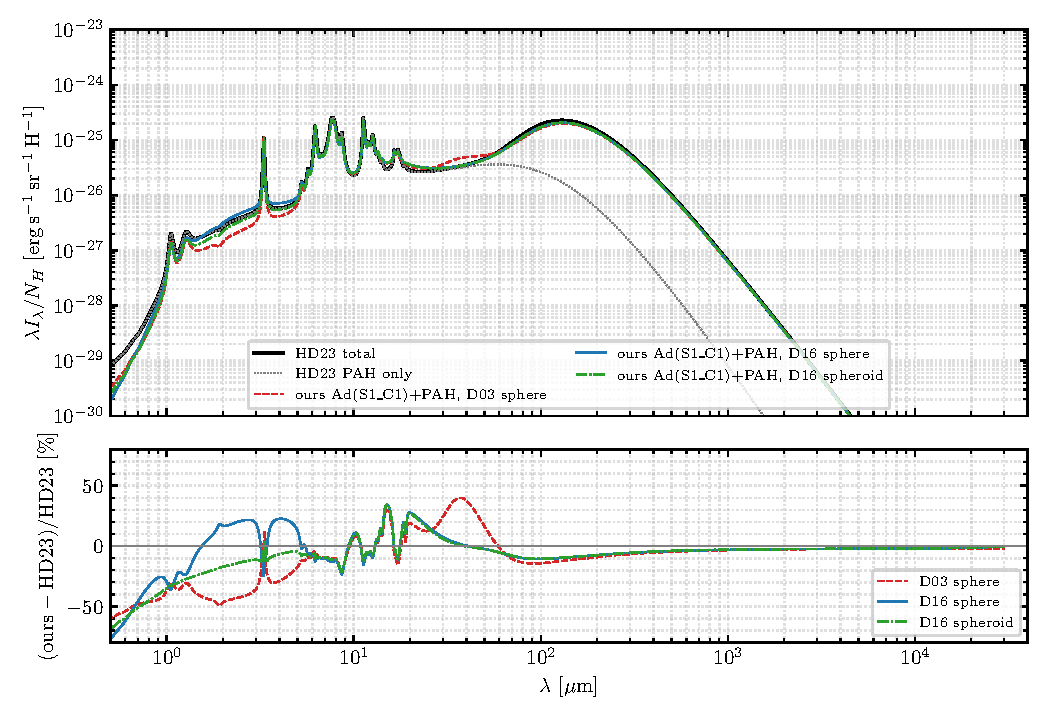
\includegraphics[width=0.95\textwidth]{figs/sed_total_d16_threeway.pdf}
\caption{Three-way comparison of the $\xi$-blend graphite source.
Top: HD23 total (black solid) and HD23 PAH-only (gray dotted) on the
release wavelength grid, plus our \texttt{S1\_C1 + PAH} totals with
three graphite-source choices for the $\xi$-blend (D03 sphere
red dashed, D16 sphere blue solid, D16 spheroid green dash-dot).
Bottom: relative residual of each total against HD23
\texttt{model\_irem.dat}. What separates the three is the PAH sub-mm:
the 300--3000\,$\mu$m PAH-only band ratio is $0.61$ for the D03 sphere,
$0.99$ for the D16 sphere and $1.05$ for the D16 spheroid. On the total
the choice matters much less, because the astrodust population carries
that band --- the residual at the \SI{130}{\micro\meter} FIR peak moves
only from $-12.3\%$ (D03 sphere) to $-9.8\%$ (D16 sphere) and $-9.5\%$
(D16 spheroid), and the $+34\%$ spike near \SI{15}{\micro\meter} is in
all three.}
\label{fig:d16_swap}
\end{figure}

\paragraph{Updated band-integrated ratios.} The table below replaces
the D03-sphere numbers above with the production D16-sphere values,
side by side with the alternative variants. ``ours / HD23'' is the
ratio of band-integrated $\int (\lambda I_\lambda)/\lambda \, d\lambda$
on the wavelength grid of the release file (\texttt{PAH\_irem.dat},
$\log U = 0.20$):

\begin{tabularx}{0.95\textwidth}{l c c c X}
\toprule
band ($\mu$m) & D03 sphere & D16 sphere & D16 spheroid & notes \\
\midrule
optical ($\lambda < 1$\,$\mu$m)         & 0.55 & 0.66 & 0.57 & absolute $\sim 10^{-28}$, negligible vs total \\
NIR (1--5\,$\mu$m)                      & 0.77 & 1.03 & 0.88 & PAH-feature region \\
PAH features (5--15\,$\mu$m)            & 0.92 & 0.91 & 0.92 & dominated by DL07 Drude profiles \\
mid-IR (15--60\,$\mu$m)                 & 1.19 & 1.06 & 1.05 & \\
FIR (60--300\,$\mu$m)                   & 0.75 & 0.96 & 0.98 & D03 keeps the original 25\% deficit \\
sub-mm (300--3000\,$\mu$m)              & 0.61 & \textbf{0.99} & 1.05 & D16 sphere essentially zero residual \\
TOTAL (0.1--3000\,$\mu$m)               & 0.96 & 0.97 & 0.97 & global agreement preserved \\
\bottomrule
\end{tabularx}

\medskip
\noindent All three columns are measurements of the present code, taken
in the same run of \texttt{docs/make\_figs.py} that draws
\autoref{fig:d16_swap}: the production run supplies the D16-sphere
column, and \texttt{./calc\_sed.x astrodust gra\_d03\_sphere} and
\texttt{./calc\_sed.x astrodust gra\_d16\_spheroid} the other two. They may
therefore be read digit for digit against each other. The D03-sphere
column here differs from the D03-sphere table earlier in
\S\ref{sec:pah}, which predates the enthalpy ghost-bin correction and
the correction of the DL07 eq.~2 cation near-IR continuum to
$\exp[-(0.1x)^2]$ and is kept there only as the record of that state.

The 40\% sub-mm under-prediction reported above (D03 sphere column)
is fully closed by the D16 swap; the residual $\sim 1\%$ in the sub-mm
band is within the expected DL07-vs-HD23 calibration noise. What is
left is in the PAH features themselves --- the 5--\SI{15}{\micro\meter}
band integrates $9\%$ low while the NIR sits $3\%$ high --- a
cross-section issue independent of the graphite source
(\autoref{sec:pah_feature_residual}).

\subsection{Residual PAH-feature strength mismatch}
\label{sec:pah_feature_residual}

After the D16 sphere swap, the remaining $\lambda < 5$\,\si{\micro\metre}
PAH residual decomposed into (i)~a smooth NIR continuum, which then
carried a $-15\%$ NIR-band deficit, and (ii)~a feature-by-feature
strength mismatch independent of the graphite source. Part~(i) no
longer holds: the 1--\SI{5}{\micro\meter} band now integrates to
$1.03\times$ HD23 rather than under-predicting it. Part~(ii) remains,
and the numbers below are a measurement of the present production code
against HD23 \texttt{PAH\_irem.dat} at $\log U = 0.20$, printed by
\texttt{docs/make\_figs.py} alongside \autoref{fig:sed_total}. A
feature's band is $\lambda_j(1 \pm \gamma_j)$ --- one Drude FWHM to
either side of the DL07 Table~1 mode centre, since a profile written in
$(\lambda/\lambda_j - \lambda_j/\lambda)$ reaches half maximum at
$\pm\gamma_j$ and so has FWHM $= \gamma_j \lambda_j$ --- united over the
modes that make up a complex, and widened to the three nearest release
grid points where the FWHM falls below the grid spacing (only the
\SI{3.3}{\micro\meter} stretch, FWHM \SI{0.040}{\micro\meter} against a
\SI{0.042}{\micro\meter} spacing). The bands contain the underlying
continuum, so these are band ratios and not continuum-subtracted feature
strengths:

\begin{tabularx}{0.9\textwidth}{l c c X}
\toprule
feature & band ($\mu$m) & ours / HD23 & \\
\midrule
\SI{3.3}{\micro\meter} aromatic C--H stretch  & 3.256--3.344   & 0.79 & largest deficit \\
\SI{6.2}{\micro\meter} C--C stretch           & 6.033--6.407   & 0.89 & \\
\SI{7.7}{\micro\meter} C--C complex           & 6.482--8.352   & 0.88 & modes $j = 11$--13 \\
\SI{8.6}{\micro\meter} C--H in-plane bend     & 8.274--8.946   & 0.79 & \\
\SI{11.3}{\micro\meter} C--H out-of-plane     & 10.967--11.693 & 0.87 & modes $j = 17, 18$ \\
12.0--\SI{12.7}{\micro\meter} duo/trio        & 11.450--13.150 & 0.93 & modes $j = 19$--21 \\
\SI{14.19}{\micro\meter} quartet              & 13.835--14.545 & 1.14 & the one band over-predicted \\
\SI{17}{\micro\meter} complex                 & 15.932--18.156 & 0.98 & modes $j = 26$--28 \\
\bottomrule
\end{tabularx}

\medskip
\noindent Every band except the \SI{14.19}{\micro\meter} quartet comes
out low, by 7--21\%, and the deficit is deepest at the two narrowest
C--H bands (3.3 and \SI{8.6}{\micro\meter}, both $-21\%$). The HD23
paper~\S3.2 states that its PAH cross sections are ``identical to those
of DL07 with the exceptions of the \SI{14.19}{\micro\meter} feature and
the \SI{17}{\micro\meter} complex, which have both been increased in
strength by 33\%''; our residuals are not consistent with that single
isolated change. Were those two bands the only difference, both would
sit $\sim 25\%$ low here, whereas the \SI{14.19}{\micro\meter} band is
14\% \emph{high} and the \SI{17}{\micro\meter} complex agrees to 2\%,
while bands HD23 says it left alone are 10--20\% low. A separate
inspection of DL07 Table 1 itself
(in the context of the SED\_v5 \texttt{QPAH\_DL07} fork from which
\texttt{sed/src/qpah.f90} descends) found that the
\SI{1.260}{\micro\meter} ionized PAH strength is
$\sigma_{\rm Ion}(4) = 0.078$ in the published table whereas a value of
$7.8 \times 10^3$ (a factor of $10^5$ larger) reproduces the publicly
distributed DL07 SED; the SED\_v5 fork uses the corrected value and
this report inherits that correction. We document the feature-by-feature
residuals here as a numerical record; a definitive resolution would
require either an independent re-derivation of the DL07 Drude
parameters or direct correspondence with the HD23 authors about which
DL07 Table 1 entries went into their \texttt{PAH\_irem.dat}
construction.

\paragraph{Mode-by-mode Drude tuning to HD23.} An empirical
mode-by-mode rescaling of the DL07 Drude parameters was fitted at an
earlier stage of this work, and closed the feature-by-feature mismatch,
as it was estimated then, to within $\pm 3\%$ at the dominant peaks
(3.3, 6.2, 7.7-complex, 8.6, 11.3-complex, 12.0--12.7-complex, 17
complex). Mode-by-mode multiplicative factors $f^{(j)}_\sigma$ for
\texttt{sigma\_neu(j)} and \texttt{sigma\_ion(j)} (and optionally
$f^{(j)}_\gamma$ for the Drude width) live as module-level public
arrays in \texttt{sed/src/qpah.f90} (toggle \texttt{use\_tuned\_pah},
default \texttt{.false.}), and the fitted values are recorded in
\texttt{sed/pah\_tune.nml}. No driver in this tree reads that file and
none takes a \texttt{pah\_tuned} argument: switching the tuning on means
setting \texttt{use\_tuned\_pah} and the two arrays from calling code,
and there is no tuned production run. The convergence path was:
(i)~three iterations of single-mode adjustment using a feature-by-feature
ratio diagnostic; (ii)~a 2-mode least-squares fit on
$j=22$ and $j=23$, which drove
$f^{(23)}_\sigma$ to the lower clamp at $0.30$ -- diagnostic for
graphite-continuum bleed into those weak features rather than a
PAH-$\sigma$ issue; (iii)~a 130-point $(\sigma_6, \gamma_6)$
brute-force grid search at the \SI{3.3}{\micro\meter}
peak to resolve the $\sigma$-vs-$\gamma$ ambiguity inherent in
that very narrow Drude profile ($\gamma_6 = 0.012$, FWHM $\approx
0.04\,\mu$m -- comparable to HD23's grid spacing of
$0.042\,\mu$m). The grid optimum is at
$f^{(6)}_\sigma = 2.00$ with $f^{(6)}_\gamma = 1.00$
(i.e., HD23 boosted only the integrated strength of the
\SI{3.3}{\micro\meter} C--H stretch; the underlying Drude width
matches DL07), with $\chi^2 = 5.0\times 10^{-4}$ over the three
nearest HD23 grid points. Pure-$\gamma$-narrow
($f_\gamma = 0.45$) and equal-boost ($f_\sigma = f_\gamma = 1.45$)
scenarios are 5--10$\times$ worse, ruling them out.
Table~\ref{tab:pah_tune} lists the final factors. The residual
$+5$--$15\%$ over-prediction at 13--\SI{19}{\micro\meter} is
attributed to the graphite continuum (it cannot be closed by PAH
$\sigma$ adjustment alone, as the LS fit demonstrated) and is
discussed further in \S\ref{sec:pah}.

Two things about Table~\ref{tab:pah_tune} need saying plainly. The
factors were fitted against the code as it stood before the enthalpy
ghost-bin correction and before the DL07 eq.~2 cation near-IR continuum
was corrected to $\exp[-(0.1x)^2]$, so they are not a fit to the
residuals tabulated above. And the estimator they were fitted to --- the
``optical-equivalent ratio'' of each feature --- was never recorded with
a band definition or a continuum-subtraction rule, so the fit cannot be
re-derived from what this tree carries. The table is kept as the record
of that fit, not as a recommended setting.

\begin{table}[h]
\centering
\small
\begin{tabular}{r r l r}
\toprule
$j$ & $\lambda_j$ ($\mu$m) & feature                  & $f^{(j)}_\sigma$ \\
\midrule
  6 & 3.300  & C--H stretch (3.3)              & \textbf{2.00} \\
  7 & 5.270  & C--H/C--C combo                 & 0.84 \\
  8 & 5.700  & C--H/C--C combo                 & 0.81 \\
  9 & 6.220  & C--C stretch (6.2)              & 0.73 \\
 10 & 6.690  & weak                            & 0.86 \\
 11 & 7.417  & 7.7 complex (a)                 & 0.79 \\
 12 & 7.598  & 7.7 complex (b)                 & 0.79 \\
 13 & 7.850  & 7.7 complex (c)                 & 0.76 \\
 14 & 8.330  & weak                            & 1.04 \\
 15 & 8.610  & C--H in-plane bend (8.6)        & 1.02 \\
 17 & 11.23  & C--H oop (solo narrow)          & 1.34 \\
 18 & 11.33  & C--H oop (solo broad, 11.3)     & 1.33 \\
 19 & 11.99  & duo                             & 1.17 \\
 20 & 12.62  & trio                            & 1.24 \\
 21 & 12.69  & trio                            & 1.22 \\
 22 & 13.48  & quartet                         & 1.06 \\
 23 & 14.19  & quartet (HD23 +33\%)            & 1.03 \\
 25 & 16.45  & C-C-C bend                      & 1.15 \\
 26 & 17.04  & C-C-C bend (HD23 +33\%)         & 1.34 \\
 27 & 17.375 & C-C-C bend                      & 1.24 \\
 28 & 17.87  & C-C-C bend                      & 1.02 \\
 29 & 18.92  & weak                            & 0.87 \\
\bottomrule
\end{tabular}
\caption{Final mode-by-mode Drude $\sigma$ multipliers applied to DL07
Table~1 to reproduce HD23 \texttt{PAH\_irem.dat} at $\log U = 0.20$
(all $f^{(j)}_\gamma$ left at $1.00$). $f^{(j)}_\sigma$ is applied
identically to \texttt{sigma\_neu} and \texttt{sigma\_ion}. Modes
not listed are kept at $f = 1$ (no change). Recorded in
\texttt{sed/pah\_tune.nml}, which no driver reads; see the text for the
configuration the fit was made in.}
\label{tab:pah_tune}
\end{table}


\section{Polarization}

Per HD23~\S3.2, the PAH track does \emph{not} contribute to polarized
extinction or emission (PAH grains are spherical in the model and not
aligned). The polarization comparison below therefore uses the
astrodust population only.

The comparison below is a \emph{verification of the T-matrix optics}
against the HD23 release, carried out by a standalone utility. In this
tree --- v1.20, the polarized branch --- the same quantity is also a
library capability: \texttt{dust\_extinction} returns the dichroic
extinction $C_{\rm pol}^{\rm ext}$ and the birefringent extinction
$C_{\rm bir}^{\rm ext}$ alongside the scalar cross sections, and the
aligned-grain scattering matrix is reached through a separate query
API. Both are documented in
\texttt{docs/sedust\_polarization\_implementation.tex}. The scalar
branch (v1.00) carries the emission and extinction API without any of
them.

For perfectly oblate spheroids with the short (symmetry) axis aligned
perpendicular to a magnetic field in the plane of the sky (the
``MPFA'' geometry of HD23 \S2.2), the maximum polarized extinction per
H atom is
\begin{equation}
\left(\frac{p_\lambda}{N_H}\right)^{\max}
= \sum_a \frac{dn_{\rm Ad}}{N_H}(a)\,
  C_{\rm pol}^{\rm ext}(\lambda, a)\, f_{\rm align}(a),
\label{eq:pmax}
\end{equation}
where
\begin{equation}
C_{\rm pol}^{\rm ext}(\lambda, a) = \frac{1}{2}\,\pi a^2\,
   \left[\Qext^{\,E\perp a}(\lambda, a) - \Qext^{\,E\parallel a}(\lambda, a)\right]
\end{equation}
is the dichroic-extinction component, and
$\Qext^{\,E\parallel a}$, $\Qext^{\,E\perp a}$ are Mishchenko's
\texttt{jori = 2} (E parallel to symmetry axis) and
\texttt{jori = 3} (E perpendicular) Q values. The alignment efficiency
$f_{\rm align}(a)$ is read from \texttt{size\_distribution.dat}
column~5.

To save the cost of a separate orientation-resolved T-matrix sweep,
\texttt{docs/make\_figs.py} reads
the HD23 release file
\texttt{q\_DH21Ad\_P0.20\_Fe0.00\_1.400.dat.gz} directly --- this file
already contains all three jori Q tables. The Q values are
interpolated in $\log a$ from the 169-point DH21 grid onto the
167-point size-distribution grid, eq.~\ref{eq:pmax} is evaluated, and
the result is compared against
\texttt{polarized\_extinction.dat}.

\autoref{fig:pol} shows the comparison. The peak value
$|p^{\max}/N_H| = 1.521 \times 10^{-23}$~\si{cm^2.H^{-1}} at
\SI{0.59}{\micro\meter} agrees with the HD23 peak
$1.520 \times 10^{-23}$~\si{cm^2.H^{-1}} at the same wavelength to
four significant figures. Mean $|$relative residual$|$ is below 0.07\%
in every band from optical to millimeter; the only outliers are at
the cross-polarization sign-flip in the deep UV where the reference
itself is going through zero. This is essentially a perfect
reproduction.

\begin{figure}[h]
\centering
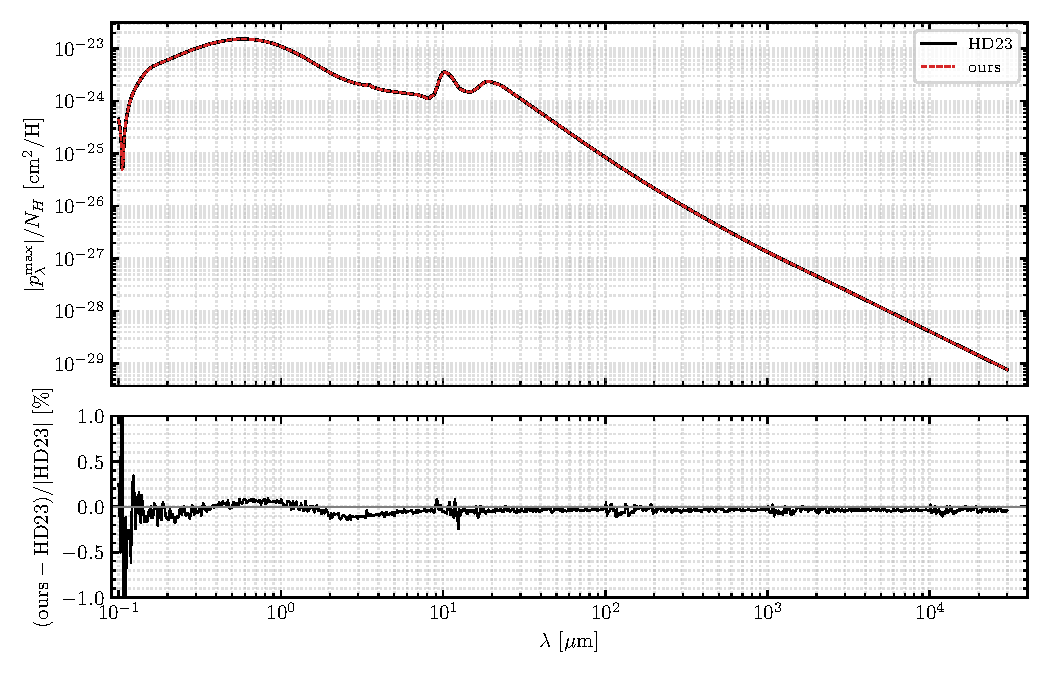
\includegraphics[width=0.9\textwidth]{figs/polarization.pdf}
\caption{Top: $|p^{\max}_\lambda|/N_H$ from HD23
\texttt{polarized\_extinction.dat} (black solid) and from
eq.~\ref{eq:pmax} evaluated on the HD23 release Q tables (red dashed).
Bottom: relative residual in percent. Peak value agrees to four
significant figures.}
\label{fig:pol}
\end{figure}


\section{Python utility (Phase G)}

A standalone Python sidecar of the single-grain SED solver is provided in
\texttt{pyutil/sed\_from\_cabs.py}. It exposes
\begin{verbatim}
   T_eq, lamI_lam = sed_equilibrium(lam_um, Cabs, J_lam)
   P, lamI_lam    = sed_stochastic (lam_um, Cabs, J_lam, T_grid, U_grain)
\end{verbatim}
with the same unit conventions and the same matrix solver as the
Fortran library. The function signature takes only what a single
3D-RT cell needs: $\lambda$, $C_{\rm abs}(\lambda)$, $J_\lambda$, and
(for stochastic mode) the enthalpy $U(T)$ on a user-chosen $T$ grid.
A one-off check extracted $\Cabs$ for a single
$a = 0.1$\,$\mu$m astrodust grain from the Fortran Q table, built the
Mathis ISRF at $U = 1.585$ and solved equilibrium: $\Teq = 17.34$~K,
comfortably in the expected ISM range and within $0.5$~K of the
Fortran-computed value for a nearby grain. That check was not kept as a
test; \texttt{pyutil/tests/} carries only
\texttt{test\_sedust\_h5.py}, which round-trips the HDF5 products.

The Python sidecar is intended for prototyping radiation-field
shapes, plotting single-grain spectra, and validating the Fortran
library on representative grains without running the full
size-distribution pipeline.


\section{Model-agnostic dust-emission library (Phase H)}
\label{sec:phaseH-library}

The two-step solver of Phase~D has been packaged into a
\emph{model-agnostic dust thermal-emission library} that a Fortran 3D
radiative-transfer (RT) code can link to compute the IR emission of a
dust mixture for an arbitrary local radiation field. The motivation is
operational: the same validated solver should serve astrodust, the
legacy DL07 silicate+carbonaceous model, and additional models (here
Zubko, Dwek \& Arendt~2004) as \emph{peers}, selected at run time rather
than hard-wired.

\paragraph{Architecture (wrap, do not move).} The numerically validated
solver core --- \texttt{sed\_grain\_loop} with \texttt{calc\_Teq} /
\texttt{calc\_P} (\texttt{p\_sub.f90}) and \texttt{qm\_solve\_grain}
(\texttt{stoch\_qm.f90}) --- is left \emph{unchanged}; the library is a
purely additive layer. Production \texttt{calc\_sed.x astrodust} and
\texttt{calc\_sed.x dl07} outputs stay bit-identical (verified byte-for-byte
at fixed \texttt{OMP\_NUM\_THREADS}). A dust model is represented by one
derived type, \texttt{dust\_model\_t} (in the new
\texttt{sed/src/dust\_model\_mod.f90}), holding the wavelength /
size / temperature grids and an array of grain \emph{populations}
(\texttt{grain\_pop\_t}, one per species and charge state, each carrying
its own size distribution, \Cabs/\Qsca, enthalpy, and Planck-integral
tables). The emission is summed into named output \emph{channels}.

\paragraph{Models as peers.} Four builders fill a \texttt{dust\_model\_t};
each sets its own optics and abundance parameters internally:

\begin{tabularx}{0.95\textwidth}{l l l}
\toprule
builder & model & channels \\
\midrule
\texttt{build\_astrodust}   & HD23 astrodust+PAH ($N_C{=}417$, D16 graphite) & \texttt{AD}, \texttt{PAH} \\
\texttt{build\_dl07}        & Draine \& Li 2007 ($N_C{=}470$, D03 graphite)  & \texttt{SIL}, \texttt{CARB} \\
\texttt{build\_zubko}       & Zubko et al.~2004 (ZDA) BARE-GR-S              & \texttt{PAH}, \texttt{GRA}, \texttt{SIL} \\
\texttt{build\_from\_files} & generic, defined by a text descriptor         & \texttt{CH1}, \texttt{CH2}, \ldots \\
\bottomrule
\end{tabularx}

\noindent The Zubko model exercises the design's generality: a neutral-only
PAH population (no charge split), component-by-component size grids, a ZDA-style
$Q$-table optics reader, and a \emph{specific-enthalpy} calorimetry source
(\texttt{sed/src/zubko\_io.f90}) --- all confined to the builder, so the
solver core is untouched. Its data (config/formula, size tables, optics,
calorimetry) is taken from the Camps et al.~2015 benchmark and copied into
\texttt{data/zubko/}.

\paragraph{Emission and solver options.} The RT code calls
\texttt{dust\_emission(m, J\_lam, lamI\_total [, lamI\_chan])} once per
cell with that cell's mean intensity on \texttt{m\%lam}; the result is
\lamIlam/\Nh\ in the HD23 convention, optionally split by channel. The
solver is chosen by \texttt{m\%stoch\_method}: \texttt{'heuristic'}
(default; the look-ahead $T$-window narrowing, fastest and
serial --- ideal inside an RT cell loop), \texttt{'draine'}
(Guhathakurta \& Draine~1989), \texttt{'qm'} (the energy-space
transition-matrix solver of \S\ref{sec:phaseE-residual-analysis}), or
\texttt{'equil'} (force every grain to its own equilibrium \Teq). Two
equilibrium-temperature options are provided for fast approximate
transfer: an equilibrium \Teq\ for each grain species and size
(\texttt{stoch\_method = 'equil'}), and a single \Teq\ for the whole mixture from the
abundance-weighted total absorption cross section
(\texttt{dust\_emission\_single\_teq}). Both conserve energy by
construction; the single-\Teq\ value for the diffuse-ISM field is
$\Teq = \SI{19.24}{\kelvin}$, with total power within $0.1\%$ of the
stochastic solve --- they differ only in SED \emph{shape} (a smooth
modified blackbody versus one carrying the PAH/NIR features).

\paragraph{Single-cell solve versus precomputed table.} For an arbitrary
field shape the single-cell exact \texttt{dust\_emission} is used. When the
cell field is a fixed reference shape scaled by an intensity $U$, a
precompute-and-interpolate path (\texttt{dust\_build\_table} /
\texttt{dust\_emission\_interp}, log--log in $U$) avoids the single-cell
solve and is exact at the grid points. The table is valid \emph{only}
for $U\times(\text{fixed shape})$: stochastic emission is a nonlinear
functional of the full $J(\lambda)$, so cells with a hardened spectrum
must use the exact solve. This caveat is documented in the API contract.

\paragraph{Extinction from the same object.} A transfer code needs
opacity as well as emission, and taking the two from different files is
how a run ends up transporting one dust model while re-emitting
another. \texttt{dust\_extinction(m, Cext, Cabs, Csca [, gbar]
[, Cpol\_ext] [, Cbir\_ext] [, albedo] [, status])} is therefore the
extinction twin of \texttt{dust\_emission}: it returns the
size-distribution-integrated cross sections per H on the model's own
grid \texttt{m\%lam}, as the plain binned sums
$C_{\rm abs} = \sum_{\rm pop}\sum_a {\rm d}n(a) C_{\rm abs}(\lambda,a)$
and likewise for $C_{\rm sca}$, with
$\langle\cos\theta\rangle = \sum {\rm d}n\,C_{\rm sca}g / \sum {\rm
d}n\,C_{\rm sca}$ and albedo $C_{\rm sca}/C_{\rm ext}$. All four
builders now carry scattering optics --- astrodust from the T-matrix
$Q$ table, DL07 from Mie on the D03 astrosilicate and graphite
dielectric functions, Zubko and the file-defined models from the
$Q_{\rm sca}$ and $g$ columns of their own tables --- so the albedo is
a physical quantity for every model, not just astrodust. Populations
that genuinely do not scatter (the astrodust PAHs, which are
Rayleigh-negligible) leave those arrays unallocated and contribute
zero. The two polarized outputs follow the same summation weighted by
the alignment efficiency, $\sum_a {\rm d}n(a) C(\lambda,a)
f_{\rm align}(a)$, and stay zero for a model with no aligned
population.

\paragraph{Linking and validation.} \texttt{make libsedust.a} produces a
static archive that an external Fortran RT links with
\texttt{gfortran -I<sed> rt.f90 libsedust.a -fopenmp}; a minimal working
driver is \texttt{sed/rt\_example/use\_dustlib.f90}. Validation: the typed path
reproduces the production astrodust and DL07 channels to machine
precision; the table interpolated at a grid point matches the direct
solve to $\sim 10^{-15}$; and the two equilibrium options conserve
energy to $0.1\%$. The complete API and usage are documented separately
in \texttt{docs/SEDust\_user\_manual.tex}.

\section{Transport optics and the ionizing band}
\label{sec:euv}

\subsection{One driver, every model}

\texttt{sed/src/calc\_kext.f90} builds a model and calls
\texttt{dust\_extinction} on it, so the curve files it writes into
\texttt{data/} \emph{are} the optics an RT host gets in memory rather
than a separately maintained product:
\begin{verbatim}
   ./calc_kext.x astrodust [euv | <lam_min in um>]
   ./calc_kext.x dl07      [ld01] [euv | <lam_min in um>]
   ./calc_kext.x mrn       [euv | <lam_min in um>]
   ./calc_kext.x zubko     [formula | table]
   ./calc_kext.x from_files <descriptor> [data_dir]
\end{verbatim}
Every product carries $\lambda$\,[\si{\micro\meter}], albedo,
$\langle\cos\theta\rangle$, $C_{\rm ext}$/H, $C_{\rm abs}$/H,
$C_{\rm sca}$/H. The first four are in the order of Draine's
\texttt{kext\_albedo} tables, so a reader written for those files parses
these unchanged; the fifth is not, being $C_{\rm abs}$/H rather than
Draine's $K_{\rm abs}$. \texttt{data/astrodust/kext\_astrodust\_MW.dat}, which is
a tracked regression reference and keeps a frozen on-disk format, adds
two more: $K_{\rm abs}$\,[\si{cm^2/g}] from the model's own dust mass
per H, and the dichroic extinction $C_{\rm pol}^{\rm ext}$/H, for eight
columns in all. Its polarized column is the sum of
eq.~\ref{eq:pmax}, written with the opposite sign convention
$C_{\rm pol}^{\rm ext} = \tfrac12\pi a^2[\Qext^{\,E\perp a} -
\Qext^{\,E\parallel a}]$: the \emph{maximum} polarized extinction,
quoted before the $\sin^2\gamma$ geometry factor and before any
turbulent depolarization, both of which a host must apply. Codes
reading only the first seven columns are unaffected.

The two Zubko routes are the same optics with two size distributions:
\texttt{formula} (the default) evaluates the ZDA log-polynomial on the
optics-table radii, \texttt{table} interpolates the distributed
\texttt{SzDist} files onto the same radii. Those files sit below the
config formula by $0.79\%$ (PAH), $1.13\%$ (graphite) and $0.41\%$
(silicate) in normalization, and are given on 24, 62 and 63 points that
must be interpolated, so the two routes differ in size-integrated
$C_{\rm ext}$ by up to $2.10\%$ (median $1.02\%$). The formula is
faithful to the ZDA model definition and is what the tracked product
uses.

\subsection{Extending the grid below the Lyman limit}

The astrodust wavelength grid is the grid of the T-matrix $Q$ table the
model was built from, and two scalar tables ship: the default
\texttt{q\_astrodust\_P0.20\_Fe0.00\_1.400.dat} on 1129 wavelengths from
\SI{0.0912}{\micro\meter}, and \texttt{..\_euv.dat} on 1762 reaching
\SI{1e-4}{\micro\meter} --- \SI{12.4}{\kilo\electronvolt}. The second is
the whole sweep; the first is that file with the wavelengths below the
Lyman limit dropped, so the two agree cell for cell over the 1129 they
share. \textbf{Given the \texttt{\_euv} table the ionizing band is inside
it}, computed the same way as the rest of it, so a host that transports
ionizing radiation reads it off the table and needs nothing more; in
particular it does not have to link \texttt{libtmatrix.a}.

\medskip
\noindent \texttt{build\_astrodust} and \texttt{build\_dl07} take an
optional \texttt{lam\_min} [\si{\micro\meter}] for a host that needs to
reach below the table it was given. Log-spaced points are then prepended from
\texttt{lam\_min} up to the table, at a step no coarser than the
table's own $\Delta\ln\lambda$ at its short-wavelength end ($0.00794$ on
the \texttt{\_euv} axis, $0.01156$ on the other),
with the requested floor placed exactly. Omitting \texttt{lam\_min}
prepends nothing, so every earlier result is bit-identical. The same is
true of the other options added at the same time --- the
\texttt{astrodust\_index\_path} of \texttt{sed\_init} /
\texttt{build\_astrodust}, and the \texttt{albedo} output of
\texttt{dust\_extinction}: absent, they change nothing. What
\texttt{lam\_min} does for astrodust depends on the table: on the
1129-wavelength one a floor below \SI{0.0912}{\micro\meter} builds a
band, while the \texttt{\_euv} table already reaches
the short end of the DH21 dielectric function itself
($1.00003\times10^{-4}$\,\si{\micro\meter}), so there every legal
\texttt{lam\_min} either falls inside the table, prepending nothing, or
below the dielectric data, where it is refused. DL07 can be
extended below either, to \SI{6.205e-5}{\micro\meter}, because the D03 optical
constants reach further than both.

\medskip
\noindent Where the ionizing-band astrodust optics come from is therefore the
same answer as for the rest of the table: the DH21 dielectric function,
solved by the T-matrix for the same $b/a = 1.4$ oblate spheroid on the
same random-orientation average, so the model changes neither
composition nor shape at the seam. Bohren--Huffman Mie for the
volume-equivalent \emph{sphere} remains available as a far cheaper
approximation, selected with \texttt{euv\_tmatrix=.false.}, and
\S\ref{sec:euv-shape} is the measurement of what that substitution
costs --- but for astrodust neither route now has a wavelength to
compute. The carbonaceous
side changes character at \SI{21.4}{\electronvolt}
($1/\lambda = 17.25\,\mu\mathrm{m}^{-1}$), where the DL07 PAH cross
section is zero by construction and graphite becomes the whole
carbonaceous absorption. There the D16 turbostratic sphere table can no
longer be used: its radius axis bottoms out at
\SI{1e-3}{\micro\meter} while the astrodust size grid starts at
\SI{3.55e-4}{\micro\meter}, and since $Q_{\rm abs}\propto a$ in the
Rayleigh limit, clamping to the table's first radius overestimates the
absorption by $10^{-3}\,\mu\mathrm{m}/a$ --- up to $2.4\times$ for the
smallest PAH the size distribution populates
(\SI{4.22e-4}{\micro\meter}). Above the cutoff the code therefore takes
graphite from the D03 dielectric functions by Mie
($\tfrac13$ parallel $+\ \tfrac23$ perpendicular), which has no radius
clamp. The unextended grid never reaches this branch
($1/0.0912 = 10.96 < 17.25$).

\subsection{The shape approximation and its two limits}
\label{sec:euv-shape}

\emph{No shipped astrodust product goes through this approximation, and
none goes through the route it is an approximation to.} The $Q$ table
covers the ionizing band, so every wavelength of every astrodust curve
in \texttt{data/} is read off the table and the on-the-fly band is
unreachable. What follows is the record of the measurement that decided
which particle that band would be solved on while it still had to be
solved on the fly, and of what would apply again if a dielectric
function ever reached further than the table built from it.

\medskip
\noindent The $Q$ table is a random-orientation T-matrix solution for a
$b/a = 1.4$ oblate spheroid, and so, by default, is the extended band.
This subsection concerns the \emph{optional} cheap route
(\texttt{euv\_tmatrix=.false.}), which replaces that spheroid by its
volume-equivalent \emph{sphere} and solves it with Mie. The
justification is \emph{not} the
anomalous-diffraction condition $|m-1|\ll1$: for this material
$|m-1| = 0.77$ at the seam and still $0.56$ at
\SI{20}{\electronvolt}. It is instead that the two ends of the size
range are governed by limits in which the shape drops out or enters as
a constant:

\begin{itemize}
  \item \textbf{Rayleigh limit (small grains).} At the seam the
        smallest populated radius has $x = 2\pi a/\lambda = 0.033$, and
        only $0.24$ at \SI{100}{\electronvolt}. The ellipsoid
        polarizability
        $\alpha_j = V(\epsilon-1)/\{4\pi[1+L_j(\epsilon-1)]\}$ contains
        the shape only through $L_j(\epsilon-1)$, and $|\epsilon-1|$
        falls from $1.86$ at \SI{13.5}{\electronvolt} to $1.10$ at
        \SI{20}{\electronvolt}, $0.28$ at \SI{40}{\electronvolt} and
        $0.061$ at \SI{100}{\electronvolt}. The depolarization factors
        drop out and the two shapes converge.
  \item \textbf{Geometric-optics limit (large grains).}
        $C_{\rm ext}\to2\times$ the orientation-averaged projected
        area, which by Cauchy's theorem is $S/4$. For $b/a = 1.4$ that
        exceeds $\pi a_{\rm eff}^2$ of the volume-equivalent sphere by
        $2.12\%$, so Mie is low by $1-1/1.0212 = 2.08\%$. The error
        converges to a \emph{constant}, not to zero.
\end{itemize}

\noindent The error therefore does not improve monotonically with
photon energy: only $a\lesssim\SI{2e-3}{\micro\meter}$ does, while
$a\gtrsim\SI{0.01}{\micro\meter}$ worsens between 13.6 and
\SI{30}{\electronvolt} before recovering to the constant $-1.9$ to
$-2.0\%$. Over the whole band and size range it stays within about
$2\%$; \texttt{sed/src/q\_astrodust.f90} tabulates it size by size.
Independently, an external review of this extension compared 28
T-matrix cells with $10\le x\le50$ at exactly
\SI{0.0912}{\micro\meter} against equal-volume Mie spheres and found
mean $(\mathrm{Mie}-\mathrm{TM})/\mathrm{TM}$ of $-1.92\%$ in
$Q_{\rm ext}$, $-1.89\%$ in $Q_{\rm abs}$ and $-1.94\%$ in
$Q_{\rm sca}$ --- the geometric-optics constant, arrived at from the
other side.

In the size-integrated curve that this route produces --- which is what
\texttt{data/astrodust/kext\_astrodust\_MW\_euv.dat} held while that route was the
one in use --- the step across
\SI{0.0912}{\micro\meter} is $-1.54\%$ in $C_{\rm ext}$ and $-1.90\%$
in $C_{\rm abs}$, \emph{smaller} than the neighboring steps of the
table's own grid ($-1.95\%$ / $-1.72\%$ and $-2.20\%$ / $-1.94\%$), so
absorption and extinction join without a visible discontinuity.
Scattering does show one: $C_{\rm sca}$ steps $+0.74\%$ where its
neighbors step $-0.39\%$ and $-0.36\%$, and the albedo $+2.31\%$
against $+1.59\%$ and $+1.39\%$ --- a seam of roughly one percentage
point, consistent with the $2\%$ shape error being carried mostly by
$Q_{\rm sca}$.

\medskip
\noindent Grain by grain, the T-matrix route removed that seam almost
entirely. Extrapolating the $Q$ table's first two wavelengths
log--log back to the last extended-band wavelength and comparing with
what the band produced there, over all 167 radii, the step in
$C_{\rm abs}$ had median $0.012\%$ and maximum $0.068\%$ for the
T-matrix, against median $1.17\%$ and maximum $15.7\%$ for the sphere.
The asymmetry parameter behaved the same way: the table returns
$\langle\cos\theta\rangle = 0$ wherever its own regime bounds place a
radius in the Rayleigh or geometric-optics limit, which the T-matrix
route reproduced exactly, while the sphere route stepped from $0.90$ to
$0$ across the seam for $a\gtrsim\SI{1}{\micro\meter}$.

\subsection{Two invariants that had to be protected}

Extending the grid must not move quantities that live in the infrared.
Two places needed explicit care.

\paragraph{The hardest photon.} The stochastic solver sets the top of
its enthalpy window from the energy of the hardest single photon a
grain can absorb. That bound was a hard-coded
\SI{13.6}{\electronvolt}, which an ionizing band makes wrong. It is now
$\max(\SI{13.6}{\electronvolt},\ hc/\lambda_{\rm hard})$, where
$\lambda_{\rm hard}$ is the shortest wavelength at which the incident
$J_\lambda$ exceeds $10^{-12}$ of its own peak
(\texttt{hardest\_photon\_energy} in \texttt{sed/src/radfield.f90},
called from \texttt{sed\_grain\_loop} and \texttt{narrow\_iterative} in
\texttt{sed\_astrodust.f90} and from \texttt{qm\_solve\_grain} in
\texttt{stoch\_qm.f90}).

\medskip
\noindent\emph{The bound is a property of the radiation field, not of the
wavelength grid.} The distinction used to be invisible for astrodust
and DL07, whose $Q$ table stopped at the Lyman limit itself:
$hc/\SI{0.0912}{\micro\meter} = \SI{13.595}{\electronvolt} <
\SI{13.6}{\electronvolt}$, so grid and field returned the same number.
It was never invisible for Zubko, whose
ZDA optics tables start at \SI{1e-3}{\micro\meter}: measuring the grid
there gives \SI{1239.8}{\electronvolt}, ninety-one times the Lyman
limit, for a Mathis field that carries no photon below
\SI{0.0912}{\micro\meter}. Carrying the astrodust table into the
ionizing band moves astrodust and DL07 into the same position and
further: their grid now starts at \SI{1e-4}{\micro\meter}, so the grid
candidate is \SI{12398}{\electronvolt} against the field's
\SI{13.595}{\electronvolt}, a factor of $912$. Every solver reads the
field, so losing the coincidence costs nothing --- but it is why the
grid-based form had to go before the table could be extended at all.

\medskip
\noindent Ninety-one times too high is not a change of physics but a
change of resolution. \texttt{umax} sets the upper edge of a
\emph{fixed} number of enthalpy bins, and the refinement loops do not
walk it back: contraction stops once \texttt{umax} reaches
\texttt{1.02*umaxlo} or \texttt{1.01*ub(jcut)}, and the loop is capped
at ten iterations, while expansion carries no such guard. Measured
through a host code with no
\texttt{lam\_min} requested at all, the residual coarseness moved the
Zubko dust temperature by \SI{+0.07}{\kelvin} in every cell, the ten
brightest SED bins by $-0.9$ to $-1.9\%$ and the emission image by up
to $5.4\%$, at $-0.08\%$ in total emitted energy
(\texttt{docs/EUV\_EXTENSION\_HOST\_REGRESSION.md}).

\medskip
\noindent The $10^{-12}$ floor is there to reject denormal and roundoff residue
in the unilluminated bins of a field handed over by a host, which an
exact $J_\lambda>0$ test would accept. It is a safe place to cut: a
component that far below the peak contributes at most that fraction of
the photon absorption rate, and allowing two decades for the run of
$C_{\rm abs}$ across the illuminated band, the enthalpy states it could
populate hold probability $\lesssim10^{-10}$ of the peak --- below the
$10^{-13}$ level at which both solvers already truncate the window. The
one-sidedness is deliberate: the loops widen a window that is too
narrow but are guarded against narrowing one that is too wide, so an
overestimated bound leaves the bins coarse where an underestimated one
is corrected as the loop runs. The ten-iteration cap bounds the
correction either way.

\medskip
\noindent Nothing in the tree ran the emission solvers on a model whose optics
grid reaches past the illuminated band, which is why the grid-based
form survived review. \texttt{sed/src/calc\_sed.f90} closes that gap
and is built by the default \texttt{make}: \texttt{./calc\_sed.x zubko euv}
heats the ZDA model on the whole ZDA grid with a Mathis field that stops at the
Lyman limit, \texttt{./calc\_sed.x zubko euv hardfield} adds a hard component below
it, and each prints the grid candidate against the field candidate ---
\SI{1239.8}{\electronvolt} against \SI{13.59}{\electronvolt} and
against \SI{370.1}{\electronvolt} respectively. The first run leaves
the bound at exactly \SI{13.6}{\electronvolt} and so reproduces what
the hard-coded constant produced; the second shows the bound following
the field up.

\medskip
\noindent A fourth site took the same quantity from the grid and was
found only after the extension. \texttt{calc\_P} in
\texttt{sed/src/p\_sub.f90} sets the lower limit of the transition
integral into the top enthalpy bin, and took it from
\texttt{lambda(1)}; \texttt{interp1} clamps below its range, so on the
old grid that integral was fed the radiation field's value \emph{at}
the Lyman limit for a band in which the field is exactly zero. It now
takes the limit from \texttt{hardest\_photon\_energy} as well.
\texttt{docs/EUV\_EXTENSION\_HOST\_REGRESSION.md} \S10 records the
defect and decomposes what its repair changed; removing those photons
moves the SED by far more than extending the grid does.

\paragraph{The Planck integrals.} $\kappa_B(T,a) = \int
C_{\rm abs}B_\lambda\,{\rm d}\lambda$ is evaluated on an internal
log-$\lambda$ grid. Spending a fixed budget of points on a widened
interval would coarsen the sampling of the range that actually carries
the integrand --- below \SI{0.0912}{\micro\meter}, $B_\lambda$ is
$\sim10^{-231}$ of its peak at \SI{288}{\kelvin} --- and would have
moved $\kappa_B$ by $\sim10^{-4}$ for a purely numerical reason. The
integration grid is therefore \emph{anchored} to the optics-table
range: its step and its sample points there are fixed, and the extra
points are prepended below. Measured with a
\SI{1.001e-4}{\micro\meter} floor: $\max|\Delta\kappa_B|/\kappa_B =
3.4\times10^{-16}$ over $T\le\SI{3000}{\kelvin}$ (and exactly zero
below $\sim\SI{2400}{\kelvin}$), and $\kappa_{\rm CMB}$ bit-identical.
The only non-zero difference is $1.1\times10^{-8}$ at the very top of a
\SI{5000}{\kelvin} grid, where the Wien tail genuinely reaches into the
extended band --- real extra emission, not a sampling artifact.

\subsection{What can be checked, and what cannot}
\label{sec:euv-refs}

\begin{tabularx}{0.98\textwidth}{@{}l l X@{}}
\toprule
author-provided data & coverage & contents \\
\midrule
Draine \texttt{kext\_albedo\_WD\_MW\_3.1\_60\_D03} &
\SIrange{1e-4}{1e4}{\micro\meter} &
$\lambda$, albedo, $\langle\cos\theta\rangle$, $C_{\rm ext}$/H,
$K_{\rm abs}$, $\langle\cos^2\theta\rangle$ \\
HD23 release (\texttt{extinction.dat}, \texttt{scattering.dat}) &
\SIrange{0.1}{3e4}{\micro\meter} &
absorption and scattering $\tau/N_H$ only; \textbf{no
$\langle\cos\theta\rangle$ product exists in the release} \\
Zubko ZDA optics tables & \SIrange{1e-3}{1e4}{\micro\meter} &
$Q_{\rm abs}$, $Q_{\rm sca}$, $Q_{\rm ext}$, $g$ per radius \\
\bottomrule
\end{tabularx}

\medskip
\noindent The HD23 release stops at \SI{12.4}{\electronvolt} --- exactly
where the extension begins. \textbf{The astrodust EUV band therefore
has no external reference at all}, and its accuracy rests entirely on
the internal argument above and on the seam being continuous. This
should be stated plainly whenever the extended astrodust curve is used.

The DL07 model, by contrast, can be compared with Draine's own
published table for the same model over the whole range. Evaluating
\texttt{data/dl07/kext\_dl07\_MW\_euv.dat} (1823 points, from
\SI{6.205e-5}{\micro\meter}) at the reference's wavelengths
and counting only points where the reference grid is no finer than ours
(elsewhere the comparison measures our grid, not our optics) gives, per
decade in $\lambda$, mean $|\Delta C_{\rm ext}|/C_{\rm ext}$ of
$0.069$--$0.86\%$, mean $|\Delta\,\text{albedo}| \le 0.0019$ and mean
$|\Delta\langle\cos\theta\rangle| \le 0.00073$. The excluded points
cluster at the X-ray absorption edges (Fe\,K, Si\,K, Mg\,K, Fe\,L,
O\,K, C\,K), which the reference still brackets more finely than our
grid resolves --- 150 of the 173 reference points in the
\SIrange{1e-4}{1e-3}{\micro\meter} decade and 201 of 233 in the next
one are dropped on that test, even though below the Lyman limit our
grid there is the DH21 dielectric function's own node list and not the
$\Delta\ln\lambda = 0.0116$ log grid it is at longer wavelengths. The
largest single
deviation, $7.9\%$ in the \SIrange{1}{10}{\micro\meter} decade, is
confined to the 6.2, 7.6 and \SI{7.9}{\micro\meter} PAH C--C features,
where Draine's 2003 table uses a different vintage of the PAH cross
sections (\S\ref{sec:phaseE-residual-analysis} documents the same
vintage split on the emission side).

\subsection{What the extension does not do}

The extension fixes the photon-energy mapping and the absorbed-energy
accounting in the ionizing band. It does \emph{not} make hard-photon
stochastic heating correct. The enthalpy grid is finite, and upward
transitions above its top are accumulated into the highest temperature
bin; for the smallest PAHs a \SI{54}{\electronvolt} photon already
exceeds $H(\SI{5000}{\kelvin})$. Nor is there any treatment of
photoionization, electron energy loss, fragmentation or PAH
destruction. The extended band should be used for extinction and for
absorbed-energy bookkeeping, not as a validated hard-EUV PAH
\emph{emission} model.

\subsection{Products}

\begin{tabularx}{0.98\textwidth}{@{}l r l X@{}}
\toprule
file (under \texttt{data/}) & rows & $\lambda$ [\si{\micro\meter}] &
what sets the short-wavelength floor \\
\midrule
\texttt{kext\_astrodust\_MW.dat} & 1129 & 0.0912--39810 &
the non-EUV $Q$-table grid \\
\texttt{kext\_astrodust\_MW\_euv.dat} & 1762 & 1e-4--39810 &
the \texttt{\_euv} $Q$-table grid: the requested floor is inside it, so
nothing is prepended \\
\texttt{kext\_dl07\_MW.dat} & 1129 & 0.0912--39810 &
the non-EUV $Q$-table grid, which DL07 shares \\
\texttt{kext\_dl07\_MW\_euv.dat} & 1823 & 6.205e-5--39810 &
the D03 dielectric functions; the shorter-reaching of astrosilicate and
graphite stops at $6.1992\times10^{-5}$ \\
\texttt{kext\_zubko\_BARE\_GR\_S.dat} & 866 & 0.08998--1e4 &
the ZDA optics table cut at the Lyman limit \\
\texttt{kext\_zubko\_BARE\_GR\_S\_euv.dat} & 1201 & 1e-3--1e4 &
the ZDA optics table itself; no extension is possible or needed \\
\bottomrule
\end{tabularx}

\medskip
\noindent No floor here is a free choice: each is the shortest
wavelength the data the model is made of actually covers, and a request
below it is refused (\texttt{status = 7} from \texttt{build\_astrodust}
and \texttt{build\_dl07}, or $6$ if the astrodust dielectric function
cannot be read at all) rather than served with a refractive index
frozen at the table boundary. The \texttt{euv} astrodust product reads
every wavelength of the \texttt{\_euv} $Q$ table, the ionizing band
included, so \texttt{euv} has nothing left to prepend; each non-EUV
product is its EUV counterpart's row subset from the Lyman limit on ---
same grid, same numbers, over the overlap. The two astrodust files also
differ in the columns they carry, the field width they are written
with, and their headers.
\texttt{kext\_astrodust\_MW.dat} is a tracked regression reference and
is reproduced byte for byte by \texttt{./calc\_kext.x astrodust}.

\medskip
\noindent Against the scalar branch (v1.00), which is the check that the
polarized branch did not disturb the scalar optics:
\texttt{kext\_dl07\_MW.dat}, \texttt{kext\_dl07\_MW\_euv.dat} and
\texttt{kext\_zubko\_BARE\_GR\_S.dat} are byte-identical;
\texttt{kext\_astrodust\_MW\_euv.dat} agrees in every number, its
header text being the only difference; and
\texttt{kext\_astrodust\_MW.dat} agrees byte for byte in its first
seven columns, the eighth being the polarized one the scalar branch
does not carry.

\medskip
\noindent The comparison that put the T-matrix in the ionizing band,
and eventually in the table, is worth keeping on the record. While the
band was still solved on the fly, the two routes agreed exactly at
$\lambda\ge\SI{0.0912}{\micro\meter}$, both reading those wavelengths
off the $Q$ table; below the seam the volume-equivalent sphere was low
in $C_{\rm abs}$ by up to $3.6\%$, high in $C_{\rm sca}$ by up to
$4.6\%$ and in albedo by up to $5.1\%$, and wrong in
$\langle\cos\theta\rangle$ by up to a factor of four at the shortest
wavelengths, while $C_{\rm ext}$ moved by $0.72\%$. Those are the
numbers that made the spheroid the default rather than the option.

\paragraph{Why the polarized column stops at the Lyman limit.}
The polarized products are computed band by band, for the wavelengths a
run actually needs --- the aligned scattering matrix is stored for five
optical bands, approximately $UBVRI$ --- and the ionizing band is not
among them. Shortward of \SI{0.0912}{\micro\meter} the dichroic and
birefringent extinction would need the EUV companion of the
orientation-resolved table, covering
\SIrange{0.0124}{0.0912}{\micro\meter}. That table is not distributed
and none is generated, and without it
\texttt{build\_Cpol} announces on \texttt{stderr} that the band is
``zero by omission, not by physics'' and leaves it at zero. Carrying
the wavelength grid into the ionizing band therefore put that zero on
disk: all $633$ rows of \texttt{kext\_astrodust\_MW.dat} below
\SI{0.0912}{\micro\meter} carry $C_{\rm pol}^{\rm ext}/{\rm H} = 0$
exactly, and nothing in the file distinguishes it from a computed
value. \emph{It is not one.} No other product carries the column at
all. When the companion
table \emph{is} present, the grid must lie inside it: an EUV block
reaching outside \SIrange{0.0124}{0.0912}{\micro\meter} is refused with
\texttt{status = 9}. (\texttt{status = 8} is the neighboring check on
the main polarized table, whose wavelength grid must sit node for node
on the model's own.) Below \SI{0.0124}{\micro\meter}
(\SI{100}{\electronvolt}) the opaque geometric-optics limit the table
relies on is itself invalid, which is why that is the floor. Measured
first-principles size integrals put the true
$|C_{\rm pol}^{\rm ext}|/C_{\rm ext}$ at $1.26\times10^{-3}$ at the
\SI{0.0912}{\micro\meter} join, rising to $3.64\times10^{-3}$ near
\SI{20.6}{\electronvolt} and decaying to $1.56\times10^{-4}$ at
\SI{100}{\electronvolt}, with the sign opposite to the optical band ---
small, but not the zero a missing table would report.

\section{Conclusions and next steps}

The pipeline reproduces HD23's published results across the
independent observables we have probed:

\begin{tabularx}{0.95\textwidth}{l l c}
\toprule
Quantity & Comparison & Result \\
\midrule
$\tau_{\rm Ad}/N_H$ vs \texttt{extinction.dat}       & all $\lambda$         & 0.47\% \\
$\tau^{\rm sca}_{\rm Ad}/N_H$ vs \texttt{scattering.dat} & all $\lambda$    & 0.68\% \\
$|p^{\max}|/N_H$ vs \texttt{polarized\_extinction.dat}   & all $\lambda$    & 0.07\% \\
PAH peak position vs \texttt{PAH\_irem.dat}              & \SI{7.67}{\micro\meter} vs \SI{7.69}{\micro\meter}    & two sig figs \\
PAH total (0.1--3000\,$\mu$m)                          & integrated            & 0.966$\times$ HD23 \\
PAH sub-mm (300--3000\,$\mu$m)                         & integrated            & 0.988$\times$ HD23 \\
\Teq\ vs independent bisection solver (167 grains)       & all $a$               & 0.14\% rms \\
SED Ad vs \texttt{astrodust\_irem.dat}                   & 30--300\,$\mu$m median & 7.57\% (under) \\
SED Ad vs \texttt{astrodust\_irem.dat}                   & \SI{133}{\micro\meter} peak & 10.06\% (under) \\
SED Ad total (0.1--3000\,$\mu$m)                         & integrated            & 0.911$\times$ HD23 \\
\bottomrule
\end{tabularx}

The astrodust extinction, scattering, and polarized extinction are
reproduced essentially exactly. The two thermal-emission observables
integrate to $0.911\times$ (astrodust) and $0.966\times$ (PAH) the
released totals, both in the direction and of the size that
Table~\ref{tab:ad_energy} attributes to the release itself. The
headline FIR-peak deficit -- $14.33\%$ with the original Mathis
field, $7.57\%$ in the current production after the corrected
Mathis 4000\,K dilution factor is applied (median over
30--\SI{300}{\micro\meter}; $10.06\%$ at the \SI{133}{\micro\meter}
peak) -- and the corresponding PAH residual ($\sim 40\%$ originally in
sub-mm, $1.2\%$ now in sub-mm and $3.1\%$ under in 30--\SI{300}{\micro\meter}) have been
the focus of an
extensive diagnostic effort that ultimately resolved the residual as
HD23's own energy non-conservation (\S\ref{sec:phaseE-resolution}).
Seven ports were implemented; each closed or ruled out a specific
candidate:

\begin{itemize}
  \item \textbf{Graphite continuum closed:} HD23 eq.~16's
        $\xi_{\rm gra}(a) \cdot C^{\rm gra}$ transition is now
        implemented (new modules
        \texttt{sed/src/q\_graphite.f90} and \texttt{sed/src/mie.f90}).
        The PAH sub-mm comparison moved from $\sim 90\%$ under to
        $\sim 40\%$ under -- about three-quarters of the gap closed.
        The rest went with the D16 turbostratic graphite swap
        (\S\ref{sec:d16-swap}): the production PAH sub-mm band now
        integrates to $0.988\times$ HD23.
  \item \textbf{\Teq\ verified:} an independent on-the-fly
        bracket--bisection solver, following Draine's method, was
        implemented. Grain-by-grain comparison shows
        rms 0.14\% agreement -- a $0.2$~K systematic in \Teq\ would
        give a $\sim 1\%$ discrepancy and is not present. \Teq\ is
        not the source of the FIR-peak deficit.
  \item \textbf{Grain-by-grain $T$-window iterative narrowing} (Draine v7
        algorithm) was ported alongside the SED\_v5 heuristic and run
        as a comparison. Band-integrated SED changes by $<0.5\%$,
        confirming that grid choice is not the source either. Both
        algorithms remain in the source and are switchable via a
        compile-time parameter for use in future work where the
        radiation field or size grid is very different.
  \item \textbf{Single-grain $C_{\rm abs}$ vs HD23 \texttt{jori=2/3}:} on
        the HD23 release grid, the random-orientation average
        $\tfrac{1}{3}Q^{\rm jori=2}+\tfrac{2}{3}Q^{\rm jori=3}$
        matches our single-grain $C_{\rm abs}$ to four significant
        figures across
        \SI{30}{\micro\meter}--\SI{30000}{\micro\meter} at
        $a = $\,\SI{0.126}{\micro\meter}. Q-table interpolation from
        the 169-point DH21 grid onto the 167-point size-distribution
        grid is therefore ruled out as a source of the FIR-peak
        deficit.
  \item \textbf{Direct jori=1 substitute (avenue 3):} the hypothesis
        that HD23 used the \texttt{jori=1} block of the release file
        directly (instead of constructing the random-orientation
        average) was tested by building a drop-in substitute Q-table
        and feeding it through the full \texttt{sed\_solve} pipeline.
        The substitution recovers
        only $\sim 4$ percentage points of the deficit (from $-15.1\%$
        to $-11.3\%$ at the FIR peak), with sign flips in adjacent
        bands. The orientation-convention hypothesis is rejected
        because \Teq\ self-consistency dampens the naive linear
        prediction.
  \item \textbf{Induced-emission factor $(1+J_\lambda/B_{\text{env}})$:}
        Draine's stimulated-emission boost was added behind a toggle
        (\texttt{use\_induced\_emission} in \texttt{sed\_astrodust\_mod})
        and tested via \texttt{./calc\_sed.x astrodust induced}. Measured
        induced$/$baseline ratio matches the analytic prediction
        (Tables~\ref{tab:induced_ratio},~\ref{tab:induced_vs_hd23}):
        $+0.000\%$ at $\lambda \le$~\SI{300}{\micro\meter},
        $+0.51\%$ at \SI{1}{\milli\meter}, $+21\%$ at
        \SI{3}{\milli\meter}, with the FIR-peak band left exactly
        unchanged. HD23 publishes \emph{net} emission, so this
        factor degrades agreement at long wavelengths and is left
        off; the toggle is retained as a cross-check.
  \item \textbf{Mathis 4000\,K dilution correction (applied):}
        Draine's reference ISRF implementation carries a 2008
        note recording the correction of the Mathis~1983 4000\,K
        dilution factor from $10^{-13}$ to $1.65\times 10^{-13}$
        (Draine textbook 2011, Table~12.1). Adopting this corrected
        value as the production default in our
        \texttt{radfield.f90~::~J\_Mathis} (toggle
        \texttt{use\_mathis\_corrected = .true.}) shifts the
        S1\_C1 FIR-peak residual from $-14.33\%$ to $-7.57\%$
        (Table~\ref{tab:mathis_c}); sub-mm from $-5.53\%$ to
        $-3.07\%$; mm from $-3.87\%$ to $-2.14\%$. The PAH
        30--300\,$\mu$m band closes from $-8.16\%$ to $-3.67\%$.
        The original-Mathis variant remains reproducible via
        \texttt{./calc\_sed.x astrodust mathis\_orig}.
\end{itemize}

The remaining $7.57\%$ astrodust FIR-peak deficit (and
$2$--$3\%$ sub-mm / mm deficit) was subsequently \emph{resolved}
by an energy-budget audit (\S\ref{sec:phaseE-resolution},
Table~\ref{tab:ad_energy}): the HD23 \emph{release} radiates $9.3\%$
(astrodust) and $3.2\%$ (PAH) more than its own released \Cabs\
absorb from the same field, whereas our pipeline conserves energy to
$0.15\%$. The deficit therefore equals HD23's own emitted-vs-absorbed
excess, not an error on our side, and this rules out \emph{both}
candidates raised above. Candidate~(i), a $U_{\rm Mathis}$ /
heating-field convention offset, cannot produce a
\emph{component-dependent} excess ($9.3\%$ astrodust vs.\ $3.2\%$
PAH) --- it would shift both components equally. Candidate~(ii), a
\Teq/size-sampling difference on our side, is excluded because the
pipeline conserves energy to $0.15\%$ when run against the
release-consistent \Cabs. The residual is an amplitude-type
inconsistency pointing to the internal \Cabs\ (or abundance
normalization) used for the \texttt{irem} tables exceeding what the
released extinction$-$scattering encode --- the same
internal-vs-released vintage difference documented for DL07spec and
the \texttt{iout} files. Draine's single-grain reference SED archive
(1395 spectra) uses LD93/D03 silicate rather than DH21
astrodust dielectric, so it verifies the stochastic-heating solver
structure (\S\ref{sec:phaseE-residual-analysis}) but is not a direct
astrodust FIR reference. Definitive attribution between internal
\Cabs\ and internal abundance would require HD23's internal
(pre-release) files.

\paragraph{Energy-space transition-matrix solver (DL01 \texttt{dbdis}).}
A third stochastic-heating method is implemented in
\texttt{sed/src/stoch\_qm.f90} ($\sim 2950$ lines of F90; module
\texttt{stoch\_qm\_mod}).  It works in enthalpy (energy) space rather
than temperature space, using mode-aware enthalpy bins and a
thermal-discrete (\texttt{dbdis}) transition matrix solved with a BiCG
sparse linear solver.  Two further cooling treatments share the same
upward rates and the same solver.  Thermal-continuous
(\texttt{dbcon}) collapses the downward rates into
the nearest-neighbor transition and so reproduces the
continuous-cooling approximation of the temperature-space GD recursion;
comparing the two isolates the cost of that approximation.
Exact-statistical (\texttt{stati}) replaces the Planck factor of the
downward rate by the microcanonical ratio of vibrational densities of
states $g_f/g_i$, counted exactly by the Beyer--Swinehart algorithm
over the mode spectrum, and pairs it with the matching
degeneracy-weighted emission kernel; the count is feasible only for
the smallest carbonaceous grains, and every other grain reverts to
\texttt{dbdis} within the same run.  Where the count overflows before
the top of the enthalpy range it is continued with the asymptotic
$d\ln g = dE/kT + d\ln(dE)$, whose coefficient is
$hc/k = 1.43877$\,cm\,K --- Draine's \texttt{dens\_states.f} carries
$1.48377$ at that one place, a digit transposition, and since the
branch is not reached for the grains the exact-statistical kernel runs
on, correcting it leaves every output of the released solver unchanged.
The
energy-space solver agrees with the production GD solver to within a
few percent across all wavelength bands and grain types, with 100\%
convergence (zero fallbacks to GD).  It is selected via
\texttt{./calc\_sed.x astrodust qm} (or \texttt{qm\_dbcon},
\texttt{qm\_stati}); the default
production method is unaffected.

The two-step solver API (\texttt{sed\_init} once, \texttt{sed\_solve}
per cell) is exercised end-to-end and is ready to be embedded in a 3D
radiative-transfer driver. Memory cost per process is $\sim 5$~MB;
wall-clock time per cell is $\sim 0.5$~s on Apple Silicon for the full
three-enthalpy-stage AD + PAH solve. The same model object now also
supplies the transport optics (\texttt{dust\_extinction}, scalar and
dichroic), and the wavelength grid now reaches into the ionizing
band; see \S\ref{sec:euv}. Three caveats are recorded there: the
astrodust extreme-ultraviolet band has no external reference,
hard-photon stochastic \emph{emission} is not yet a solved problem, and
the polarized optics stop at the Lyman limit, the ionizing band being
outside the wavelengths those products are made for.

\end{document}
